%==========================================================================
% DOCUMENT PREAMBLE
%==========================================================================
\documentclass[AER]{AEA}

% Note: you may use either harvard or natbib (but not both) to provide a wider
% variety of citation commands than latex supports natively. See below.

% Uncomment the next line to use the natbib package with bibtex 
\usepackage{natbib}
\usepackage{graphicx}
\usepackage{hyperref}
% \usepackage{caption} % <-- Removed as requested

% --- FIXES START HERE ---
% Added packages for better tables
\usepackage{booktabs}  % Required for \toprule, \midrule, \bottomrule
\usepackage{longtable} % Required for the longtable environment
% --- FIXES END HERE ---


% This command determines the leading (vertical space between lines) in draft mode
% with 1.5 corresponding to "double" spacing.
\draftSpacing{1.5}

%==========================================================================
% DOCUMENT BEGINS
%==========================================================================
\begin{document}

%--------------------------------------------------------------------------
% TITLE AND AUTHOR INFORMATION
%--------------------------------------------------------------------------
\title{Quantifying Investor Sentiment with Multimodal Data in the Chinese Stock Market}
\shortTitle{Multimodal Investor Sentiment}
\author{Xiaobin Liu and Yi Yu\thanks{Liu and Yu contributed equally to this work. Author order is alphabetical. Liu: Associate Professor, Lingnan College, Sun Yat-sen University (\href{mailto:liuxb53@mail.sysu.edu.cn}{liuxb53@mail.sysu.edu.cn}). Yu: M.S.\ in Data Science student, New York University (\href{mailto:yy5919@nyu.edu}{yy5919@nyu.edu}); B.A.\ in Economics, Lingnan College, Sun Yat-sen University (2024). All remaining errors are our own.}}
\pubMonth{April}
\pubYear{2026}
\pubVolume{1}
\pubIssue{1}

%--------------------------------------------------------------------------
% ABSTRACT
%--------------------------------------------------------------------------
\begin{abstract}
Using a 12-year sample of 245{,}000+ Sina Finance news articles paired with daily Chinese A-share index returns (2014--2026), we document a \emph{state-dependent and time-varying} in-sample predictive association between news photo pessimism and short-horizon market returns. Image-based pessimism (\textit{PhotoPes}, ViT-extracted) on the retail-driven ChiNext Composite is significant in 2014--2017 ($\hat{\beta}=-0.00172$, $t=-2.32$), undetectable through 2018--2023 ($|t|<1$ in both 3-year sub-periods), and partially recovering in 2024--2026 ($t=-1.88$); the full-sample headline ($|t|=2.81$, raw $p\approx 0.005$) is therefore the average of two outer sub-periods of strength and a quiet middle. Within high-volatility states, both \textit{PhotoPes} and the text-based pessimism index \textit{TextPes} carry incremental predictive content, with effect strength scaling along a retail-density gradient: the cross-sectional ranking across five indices is monotonically aligned with each of three independent retail-density proxies (the proxies themselves agree at Spearman $\rho \in [0.90, 1.00]$). An expanding-window OLS forecast under strictly causal rolling-window standardization yields out-of-sample $R^2_{OOS}=0.29\%$ on the ChiNext (one-sided MSPE-adjusted $t=2.17$, $p=0.015$); an ex-ante regime-conditional version raises the regime-active magnitude to $R^2_{OOS}=0.58\%$, but on the small regime-active subsample ($N=215$) the corresponding Clark--West $t$-statistics on all five indices fall in the range $[0.89, 1.39]$ and none clears conventional significance, so the regime-conditional finding is best read as ``consistent with but underpowered to confirm.'' The headline ChiNext effect is robust to controls for Amihud illiquidity, news volume, the Tetlock-style orthogonalization of \textit{PhotoPes} with respect to \textit{TextPes}, and trailing 5/10/20/60-day cumulative-return controls; it is null on a sentiment-free image-count placebo. We additionally report a negative cross-market replication of \citet{obaid2022picture}: the same construction generates a Sharpe gap not statistically distinguishable from zero under stationary block bootstrap (CI invariant across block lengths $\{5, 14, 22\}$) and is fully eroded by realistic Chinese A-share frictions ($\sim$17 bps round-trip). The paper is positioned as evidence on state-dependent visual-sentiment predictability concentrated in retail-driven indices, not as a tradable claim.
\end{abstract}
\JEL{G12, G14, G41}
\Keywords{Investor sentiment, Behavioral finance, Machine learning}

%--------------------------------------------------------------------------
% MAIN CONTENT BEGINS
%--------------------------------------------------------------------------
\maketitle

In recent years, investor sentiment, as a significant research direction in behavioral finance, has garnered considerable attention from the academic community due to its widespread impact on market fluctuations and investor behavior. \citet{tetlock2007giving} argued that investor sentiment not only directly affects market returns and trading volumes but also has a significant effect on market volatility, especially during periods of market panic or intense fluctuation. Quantifying investor sentiment is a key focus in financial research. In existing studies, scholars have mostly focused on quantifying the sentiment of textual content from sources like news articles and social media data, using Natural Language Processing (NLP) tools to construct text-based sentiment indicators to study the relationship between sentiment changes and market returns. These studies, primarily based on data sources from news text, have revealed a significant correlation between negative news and a decline in market returns. However, a research framework that relies solely on textual data has certain limitations and cannot fully capture the complex characteristics of investor sentiment.

With the diversification of information dissemination media, images, as an important component of news, can quickly convey complex information due to their intuitive, vivid, and lively nature, and they demonstrate a stronger effect in evoking emotions than text. The research of \citet{garcia1991eyes}, using eye-tracking technology to analyze how readers read newspapers, found that visual elements, represented by images, are typically the first content that readers notice and can attract their attention faster than words. However, the role of images in financial sentiment analysis has not been fully explored, and research on the relationship between image sentiment and financial markets is relatively scarce. \citet{obaid2022picture} utilized machine learning techniques to classify the sentiment of news images and constructed a photo pessimism index (PhotoPes) to study the impact of image sentiment on market behavior. This research demonstrated the importance of image sentiment in sentiment quantification studies, but its scope was limited to the U.S.\ market (Wall Street Journal photos, CRSP returns), with little research involving the Chinese stock market.

In the U.S.\ market setting documented by \citet{obaid2022picture}, image-based and text-based news sentiment are reported as substitutes: once image pessimism is included in a joint forecast, the contemporaneous text signal absorbs little additional predictive content. The state-dependent amplification of \emph{text-based} sentiment in turbulent markets has been established by \citet{garcia2013sentiment} on Depression-era Wall Street Journal columns and by \citet{da2015fears} on Google-search FEARS indices that load on high-VIX days; the present paper extends this state-dependence story to the visual modality, in a Chinese setting, and decomposes it cross-sectionally by retail density. The U.S.\ news-readership and ownership structure also differs systematically from China's. The Chinese A-share market is dominated by retail investors \citep{liu2019size,jones2025retail}, has substantial limits to arbitrage including binding short-sale constraints \citep{stambaugh2012short,han2022chinese}, and exhibits a much wider cross-sectional dispersion in retail-density across listed indices than U.S.\ index families. These structural differences plausibly shift not the existence but the \emph{cross-sectional and state-dependent geometry} of the visual-versus-textual sentiment relationship --- a question that has not been directly examined in this market.

\paragraph{Empirical questions.} We test three related questions: (i) in the Chinese A-share market, do image and text sentiment carry distinguishable predictive content for index returns, or is one modality a transformation of the other; (ii) does the strength of either signal vary with market volatility states; and (iii) if state dependence exists, does the cross-sectional ranking of effect strength across indices align with independent retail-density measurements --- that is, does a \emph{retail-density to modality-sensitivity} transmission have direct empirical support?

\paragraph{Empirical design.} We employ a three-dimensional design. The \emph{index} dimension covers five Chinese A-share indices spanning the retail-density gradient: the institution-dominated CSI 300 and SHCOMP, the mid-cap SZCOMP and CSI 500, and the retail-driven ChiNext Composite. The \emph{state} dimension partitions trading days by 20-day rolling SHCOMP volatility into top-quartile (high-stress) versus the rest. The \emph{modality} dimension contrasts \textit{PhotoPes}, a daily aggregate built from a Vision Transformer trained on the \citet{you2015robust} Twitter sentiment corpus and applied to Sina Finance news photos, with \textit{TextPes}, built from the Erlangshen-Roberta-110M Chinese sentiment model applied to Sina Finance headlines and articles. Empirical support for the cross-sectional differential-sensitivity claim comes from consistent ordering of effect strength across the five indices and three retail-density proxies (turnover, inverse free-float market capitalization, retail account share). Empirical support for the state-dependence claim comes from the high-versus-low volatility regime contrast.

\paragraph{Contributions.} Our contribution complements rather than displaces the existing literature; the combination of three pieces is, to our knowledge, new:
(i) we record visual and textual investor sentiment in the Chinese A-share market on a 12-year sample (2014--2026, $\sim$245{,}000 articles and 572{,}000 photographs), extending the US-focused multimodal-sentiment literature to a setting with materially different microstructure and investor composition;
(ii) we document that, in contrast to the substitute relationship reported by \citet{obaid2022picture} for the U.S., the Chinese setting exhibits cross-sectional differential sensitivity in which both modalities deliver incremental and largely independent predictive content (84\% of \textit{PhotoPes} variance is orthogonal to \textit{TextPes}; the Tetlock-style residual remains 5\%-significant on the ChiNext);
(iii) we anchor the cross-sectional pattern to a measurable consistency-of-rank pattern: the ordering of effect strength across the five indices aligns (Spearman $\rho \in [0.90, 1.00]$ across $N=5$ indices) with three independent retail-density proxies, and the headline ChiNext effect is robust to Amihud illiquidity, news-volume, and news-activity placebo controls. We acknowledge that with only five cross-sectional observations this is a suggestive rank pattern rather than a quasi-experimentally identified mechanism; a stock-level interaction extension is left for future work.

\paragraph{Negative cross-market replication.} An independent and informative finding deserves stand-alone mention: in U.S.\ data, \citet{obaid2022picture} report a statistically significant five-factor alpha for a long/short/neutral signal-thresholded rule built from their PhotoPes signal. In our Chinese A-share setting, the same construction produces a gross-of-cost Sharpe gap that is not statistically distinguishable from zero under stationary block bootstrap (95\% percentile CI $[-0.75, +0.97]$, one-sided $p=0.39$) and is fully eroded by approximately 17 basis points of round-trip transaction costs --- well within the realistic Chinese A-share retail trading-cost range. The honest interpretation is a transaction-cost-decomposition statement, not a behavioral-arbitrage claim: the full-sample standardized coefficient $|\hat\beta| \approx 0.00125$ per day on the ChiNext (the high-volatility-subsample coefficient is 2.6$\times$ larger but is realized on only 25\% of days) is too small in absolute terms for any natural execution to overcome 17~bps of round-trip frictions, and the negative tradability finding is therefore informative as a boundary on the economic magnitude rather than as a test of the \citet{shleifer1997limits} ``limits of arbitrage'' channel (the rule under test is a quantitative-fund-style 5-day-rebalanced long/short signal, not a retail-trader arbitrage). Statistical predictability concentrated in retail-driven indices need not, and in our setting does not, translate into tradable returns once realistic frictions are imposed.

\paragraph{Multiple-testing.} Following \citet{harvey2016cross}, we report Bonferroni-adjusted family-wise thresholds at three plausible family sizes ($m \in \{5, 25, 50\}$). The headline ChiNext result clears the $m=5$ threshold (the per-test $p<0.010$ appropriate when the lag is borrowed from prior literature, as in the present paper from \citet{obaid2022picture}) at the 5\% family-wise level, but does not survive the more conservative $m=25$ family. We adopt $m=5$ as the primary reading and report $m=25$ and $m=50$ as alternatives.



%==========================================================================
% SECTION: LITERATURE REVIEW
%==========================================================================
\section{Literature Review}

\subsection{Theoretical Foundations of Investor Sentiment}

Traditional financial theory, centered on the \textit{Efficient Market Hypothesis (EMH)}, posits that asset prices fully reflect all available information, and market participants are rational actors with complete information-processing capabilities. However, frequent market anomalies, such as price bubbles and excessive volatility, are difficult to explain within this traditional framework. Behavioral finance emerged as a response, integrating psychological insights into financial research and arguing that investors' cognitive biases and emotional fluctuations are significant factors causing markets to deviate from fundamentals.

In the early development of behavioral finance, the \textit{noise trader theory} proposed by \citet{de1990noise} laid the theoretical groundwork for investor sentiment research. This theory suggests the existence of a group of irrational ``noise traders'' who trade based on sentiment rather than fundamentals, causing asset prices to deviate from their intrinsic values. Crucially, even the presence of rational arbitrageurs cannot fully counteract the influence of noise traders, as arbitrage activities face numerous constraints. Furthermore, the theory indicates that the additional risk introduced by noise traders---\textit{noise trader risk}---deters arbitrageurs from taking sufficiently large positions, even when they know an asset is mispriced.

Building on noise trader theory, \citet{shleifer1997limits} systematically elaborated on the \textit{limits to arbitrage} theory, further explaining the mechanisms through which irrational behavior can persistently affect asset prices. They pointed out that the main constraints faced by arbitrageurs include fundamental risk, noise trader risk, and implementation costs. These factors collectively prevent arbitrage activities from immediately eliminating market mispricing. The limits to arbitrage theory provides a key mechanical explanation for how sentiment influences asset prices, namely that the interaction of market frictions and investor sentiment produces lasting price deviations.

\citet{baker2007investor} developed a complete analytical framework for the impact of investor sentiment on asset pricing based on the preceding theories. They emphasized that the influence of investor sentiment varies systematically across different assets, having a greater impact on those that are more subjective to value and harder to arbitrage. Such assets typically include new-economy firms, loss-making companies, high-growth firms, and high-volatility stocks. This research not only revealed the intrinsic link between asset characteristics and sentiment sensitivity but also provided a clear direction for subsequent empirical studies.

The theory of investor sentiment provides a systematic framework for explaining irrational market phenomena. It not only clarifies how sentiment factors influence market prices through noise traders but also reveals how the limits to arbitrage mechanism allows these effects to persist, and it identifies the asset characteristics and market conditions under which sentiment has the greatest impact. As research has deepened, these theories have offered new perspectives for understanding market volatility and investment behavior.

\subsection{The Evolution of Sentiment Quantification Methods}

While investor sentiment theory provides a framework for understanding market irrationality, accurately quantifying sentiment has been a long-standing challenge. With advancements in research and technology, sentiment quantification methods have evolved significantly, moving from single indicators to multivariate integration and from indirect inference to direct measurement.

Early research primarily used market technical indicators as proxies for sentiment. \citet{lee1991investor} used the closed-end fund discount as a sentiment indicator, finding that its fluctuations could predict the returns of small-cap stocks. Other commonly used market indicators include trading volume, IPO volume and first-day returns, and option-implied volatility. Although these indicators provide indirect measures of sentiment, they each have limitations and cannot fully capture the multidimensional nature of sentiment.

To overcome the limitations of single indicators, \citet{baker2006investor} constructed a composite sentiment index by combining multiple market indicators using \textit{principal component analysis}, significantly improving the comprehensiveness of sentiment measurement. This innovative method was subsequently widely adopted and extended, becoming a major milestone in sentiment quantification.

The application of text analysis techniques marked a major advancement in sentiment quantification. \citet{tetlock2007giving}, through the textual analysis of a Wall Street Journal column, was the first to systematically demonstrate that media pessimism could predict market performance, opening a new path for sentiment research. Addressing the limited accuracy of general-purpose dictionaries in a financial context, \citet{loughran2011liability} developed a specialized financial dictionary, which substantially improved the accuracy of sentiment analysis in financial texts and laid the foundation for subsequent research.

With the rise of the internet, the sources of sentiment data further expanded. \citet{bollen2011twitter} analyzed public mood using Twitter data, finding that changes in specific mood dimensions could predict the Dow Jones Industrial Average. Similarly, \citet{chen2014wisdom} analyzed investor opinions on the Seeking Alpha website, demonstrating that content from such specialized social media platforms contains valuable predictive information. These studies not only expanded the sources of sentiment data but also improved the real-time availability and granularity of sentiment measurement. Concurrently, with the increased availability of search engine data, investor attention became an important dimension of sentiment research. \citet{da2011search} used the Google \textit{Search Volume Index (SVI)} to measure investor attention, finding that it could predict short-term price pressure and long-term return reversals.

Text analysis methods also evolved from simple word frequency counts to complex machine learning models. As machine learning technology advanced, methods such as \textit{Support Vector Machine (SVM)} and \textit{Decision Trees} were widely applied to sentiment analysis. \citet{pang2008opinion} systematically compared the performance of different machine learning algorithms in text sentiment classification, demonstrating that SVM has a distinct advantage in handling high-dimensional feature spaces. Similarly, \citet{antweiler2004all} applied machine learning methods to analyze information from online forums, successfully predicting market volatility and laying the groundwork for computer-assisted sentiment analysis.

\subsection{Visual Information and Investor Sentiment}

Research in psychology and neuroscience provides strong support for the unique advantages of visual information in evoking and conveying emotions. Through mechanisms such as dual-system thinking and risk-as-feelings, this advantage significantly impacts investment decisions. Although research on visual sentiment in finance is still in its early stages, existing evidence suggests that images in financial news contain valuable emotional information that can systematically influence market performance. This research direction holds vast potential for development and significant practical importance.

Psychological studies show that visual information processing is characterized by speed, directness, and emotional intensification. \citet{powell2015visual} confirmed through comparative experiments that, compared to purely textual information, image stimuli can elicit stronger and more lasting emotional responses, which are often independent of rational cognitive processes. The constructivist view proposed by \citet{lindquist2012brain} suggests that emotional experiences are generated through the synergistic action of multiple basic psychological operations. Visual stimuli can act as inputs to trigger this construction process, but the formation of emotion involves the joint participation of both automatic and controlled cognitive processes.

These characteristics of visual information processing align closely with the \textit{Dual-System Theory} proposed by \citet{kahneman2011thinking}. According to this theory, human thinking involves two systems: System 1 (fast, automatic, and emotionally driven) and System 2 (slow, rational, and effortful). Visual information is primarily processed by System 1, thus enabling it to rapidly induce emotional reactions, whereas textual information relies more on the rational analysis of System 2. This difference is particularly important in the financial market environment, where investors in a fast-paced market often rely on System 1 to make decisions.

The \textit{risk-as-feelings hypothesis} by \citet{loewenstein2001risk} further reinforces the importance of visual information in investment decisions. This hypothesis posits that when faced with risky decisions, people often make judgments based on immediate emotional responses rather than rational calculations. Because visual information has a strong capacity to elicit emotions, it can significantly influence investors' risk perception and subsequent decision-making, especially in highly uncertain market environments.

Although the emotional effects of visual information have been extensively studied in psychology, its application in the financial domain is still an emerging field. Early financial research focused mainly on the informational content of charts and pictures in corporate annual reports, with even more limited research on the impact of images in financial media.

The visual-sentiment literature has expanded rapidly since \citet{obaid2022picture}. Three follow-up studies in \emph{Finance Research Letters} extend the photo-pessimism measure to (i) 37 international equity markets, where the effect is stronger in smaller and more retail-driven markets \citep{frl2022photo37}, (ii) the cryptocurrency market \citep{frl2023crypto}, and (iii) the segment of sustainable/ESG stocks \citep{frl2025sustainable}. \citet{ren2025investor} apply few-shot deep metric learning (DeepEMD) to news photographs, recovering a delayed return effect that is stronger for small-cap stocks. \citet{gu2026giffluence} move from static photographs to animated GIFs on social media, documenting a multi-week return reversal pattern that suggests visual sentiment carries information beyond the news-photo channel. Taken together, this literature establishes visual sentiment as a robust signal across asset classes, markets, and visual-content types, which directly motivates the present study's extension to the Chinese A-share market.

\subsection{The Application of Deep Learning in Financial Sentiment Analysis}

The rapid development of deep learning technology has brought transformative changes to financial sentiment analysis, greatly enhancing the accuracy and efficiency of processing unstructured data. This section will systematically explore the progress of deep learning applications in financial sentiment analysis, with a particular focus on breakthroughs in text analysis, image analysis, and multimodal fusion.

In the field of text sentiment analysis, deep learning methods have shown significant advantages over traditional approaches. \citet{peng2015leverage} were among the first to apply word embeddings and deep neural networks to financial news analysis, predicting stock price movements by integrating news text information and significantly improving prediction accuracy compared to traditional methods that rely solely on historical price data. Subsequently, \citet{kraus2017decision} combined Long Short-Term Memory (\textit{LSTM}) networks with transfer learning to analyze financial disclosure documents, demonstrating the superiority of deep learning methods in capturing long-term dependencies in text and predicting market reactions, while also addressing the issue of insufficient labeled data in the financial domain.

The emergence of pre-trained language models marked a major breakthrough in text sentiment analysis. The BERT (\textit{Bidirectional Encoder Representations from Transformers}) model proposed by \citet{devlin2018bert} achieved groundbreaking performance on multiple natural language processing tasks through large-scale unsupervised pre-training and a bidirectional context encoding mechanism. In its application to finance, \citet{yang2020finbert} developed the FinBERT model based on BERT, which was pre-trained on financial texts, further improving the accuracy and domain adaptability of financial text sentiment analysis.

Compared to text analysis, image sentiment analysis in finance started later but has developed rapidly. The introduction of deep learning has significantly enhanced the capabilities of image sentiment analysis. \citet{you2015robust} were the first to apply a \textit{Convolutional Neural Network (CNN)} to large-scale image sentiment classification, achieving a substantial increase in accuracy. In a specific application to financial image analysis, \citet{obaid2022picture} used the Google Inception (v3) CNN model to analyze the sentiment of financial news images, demonstrating the effectiveness and applicability of deep learning in this specialized field.

In recent years, the emergence of the Vision Transformer (\textit{ViT}) has marked a new phase in image analysis technology. The ViT model, proposed by \citet{dosovitskiy2020image}, abandoned the convolutional operations of traditional CNNs and directly applied the Transformer architecture to image processing, showing excellent performance in capturing global information and long-range dependencies. Although the application of ViT in financial image sentiment analysis is still in its infancy, its powerful expressive capabilities and flexibility signal great potential for future applications.

Multimodal fusion is an important direction in financial sentiment analysis, aiming to simultaneously analyze and integrate information from different modalities to obtain a more comprehensive sentiment representation. The research by \citet{obaid2022picture} is a significant attempt at multimodal sentiment analysis in finance. They not only analyzed image sentiment but also studied its relationship with text sentiment, finding that the two have a substitute, rather than complementary, relationship in predicting market returns. This multimodal analysis approach offers a new perspective for a comprehensive understanding of market sentiment.

A parallel body of work develops large-scale text-based sentiment indices using progressively more sophisticated NLP. \citet{tetlock2008giving} use the Wall Street Journal to quantify firm-level sentiment and document predictive content for fundamentals. \citet{manela2017news} construct news-implied volatility (NVIX) from front-page WSJ articles and predict the equity premium; this is the closest U.S.\ text-based predictor against which our \textit{TextPes} indicator is benchmarked. \citet{calomiris2019news} extend the topic-model approach to 51 international markets, documenting that news topics drive both risk and returns globally. \citet{ke2019predicting} use sentence-level word embeddings and document cross-sectional return predictability at the firm level. \citet{jiang2021manager} aggregate firm-level manager sentiment from earnings calls and document predictive content for aggregate market returns --- methodologically the closest existing precedent for our daily-aggregate sentiment-predicts-aggregate-returns design.

Among visual-sentiment work in finance, the closest U.S.\ analogs to our paper remain \citet{obaid2022picture} for the photo-pessimism construction itself and the FRL extensions \citep{frl2022photo37,frl2023crypto,frl2025sustainable} for cross-market replication. None of these studies, however, addresses the combination of image classification, market-level sentiment, and cross-sectional dispersion in retail share that our paper documents in the Chinese A-share setting.

Although the application of deep learning in financial sentiment analysis is promising, it still faces several challenges, such as a lack of model interpretability, high costs of data quality and annotation, and domain specificity. However, with continuous technological advancements, these challenges are gradually being addressed. Deep learning has brought revolutionary changes to financial sentiment analysis, from pre-trained language models for text processing to the Vision Transformer for image analysis, and multimodal fusion techniques, all of which have greatly enhanced the precision and scope of financial sentiment quantification.

\subsection{Research on Investor Sentiment in the Chinese Stock Market}

As the world's second-largest stock market, China's unique market mechanisms, investor structure, and information environment suggest that sentiment factors may play a more critical role. This section will systematically review the main progress of research on investor sentiment in the Chinese stock market, explore sentiment quantification methods with Chinese characteristics, and analyze the differential impact of sentiment factors.

Retail investors are more active in the Chinese stock market compared to other markets, a characteristic that makes the market more susceptible to sentiment. The research by \citet{kumar2006retail} shows that in markets with a high proportion of retail investors, the impact of investor sentiment on stock returns is more significant, and the trading behavior of retail investors often exhibits stronger co-movement, thereby amplifying the impact of sentiment shocks on the market. This influence is not only reflected in returns; \citet{foucault2011individual} further confirmed a significant positive correlation between the trading activity of retail investors and market volatility, indicating that the emotional fluctuations of retail investors may be an important source of excessive market volatility.
However, the impact of retail sentiment differs significantly from that of institutional investors. Research by \citet{JCYJ201403008} on the Shanghai Stock Exchange A-share market revealed this: institutional investor sentiment has predictive power for future market performance, whereas individual investor sentiment does not, indicating a fundamental difference in the quality of sentiment between different types of investors.

An important innovation in Chinese market sentiment research is the use of data from local internet platforms. \citet{JJGA201601015} combined text mining techniques and the \textit{Baidu Index} to construct an investor sentiment index by analyzing information from CSSCI journals on CNKI and Sina Weibo topics. \citet{JCYJ201804005} used posts from Eastmoney's Guba forums, employing a Naive Bayes method to construct a sentiment indicator that incorporates both bullish/bearish expectations from stock reviews and investor attention. The study found that while overall investor sentiment had no predictive power for the stock market, sentiment from stock reviews during non-trading hours before the market open could predict the opening price, providing new evidence for understanding the behavior of Chinese retail investors. Similarly, \citet{wen2019retail} used the Baidu Search Index as a proxy for retail investor attention, revealing a positive correlation between investor attention and future stock price crash risk, a relationship that is particularly pronounced in firms with high information opacity and low analyst coverage.

The media plays a unique role in the transmission of sentiment in the Chinese market. \citet{JRYJ201509012} constructed a tone indicator for media reports on IPO companies before their listing and found a significant negative correlation between negative media tone and the IPO underpricing rate. This suggests that media reports directly influence investor sentiment, which in turn affects market pricing efficiency. They also revealed that issuing companies and underwriters intentionally use media promotion to guide investor sentiment, demonstrating the special function of the media as a tool for sentiment guidance. Similarly, \citet{GLSJ202101014}, using machine learning-based text analysis, studied the contagion effect of media sentiment. They found that optimistic media sentiment significantly influences the optimistic bias of analyst forecasts and is transmitted to the market through two channels: ``limited analyst attention'' and ``investor sentiment,'' ultimately affecting stock price volatility and tail risk. These findings collectively confirm the key role of the media in the formation and transmission of sentiment in the Chinese market.

A complementary strand of work focuses on the institutional features that magnify sentiment effects in China. \citet{liu2019size} construct a Chinese version of the size and value factors and demonstrate that the standard Fama--French three-factor model requires non-trivial modification to fit the A-share market, providing a benchmark against which the CUFE-distributed Fama--French \citeyearpar{fama1993common} three factors used in our portfolio analysis can be compared. \citet{jones2025retail} document that the order-flow imbalance of retail investors carries strong predictive content for future cross-sectional returns in China, providing direct micro-level evidence for the channel through which sentiment-laden news can move prices. \citet{han2022chinese} examine 62 cross-sectional anomalies and find that anomalies are concentrated in stocks with binding short-sale constraints and during high-sentiment periods, consistent with the \citet{stambaugh2012short} mechanism in a Chinese setting.

The most directly comparable contemporaneous study is \citet{zhang2025multimodal}, who construct multimodal sentiment indices using text and photographs scraped from chinanews.com (the website of the state-owned China News Service) over 2015-01-01 to 2022-12-31. Our paper differs along four axes:
(i) \emph{Sample length and regime coverage.} Our 2014-01-02 to 2026-04-10 sample (2{,}982 trading days) extends roughly 3.5 years beyond theirs and is, to our knowledge, the only Chinese multimodal-sentiment study to date that covers the post-2022 regulatory tightening and the 2024--2026 retail-investor recovery phase, both of which fall outside their data window. The structural-stability analysis in Section~\ref{sec:break_test} shows that the predictive coefficient is statistically zero through 2018--2023 and partially recovers in 2024--2026 --- a phenomenon that, by construction, cannot be observed in their sample.
(ii) \emph{Image backbone.} We use a Vision Transformer to remain methodologically anchored to the most recent generation of computer-vision models, while \citet{zhang2025multimodal} use Google Inception~(v3).
(iii) \emph{Data source.} We collect from Sina Finance, a commercial financial-news portal that aggregates content from multiple newswires and is, by traffic, the most-read financial portal among Chinese retail investors. They collect from chinanews.com, a state-owned newswire's website dominated by official-agency reporting. The two sources have substantially different content distributions; Sina Finance is therefore the more natural channel through which sentiment-driven retail trading is plausibly transmitted.
(iv) \emph{Research question.} They construct sentiment for stock-selection and industry-level asset pricing on CSI~300 constituents; we focus on aggregate market-index return predictability across five Chinese equity indices spanning large- to small-capitalization segments.
\citet{ren2025investor} similarly study image-based investor sentiment but apply few-shot learning to a U.S.\ NYT-image sample, leaving a clear gap for systematic ViT-based analysis on Chinese-language news media that this paper fills.

Despite significant progress in research on Chinese market sentiment, the methods still primarily rely on text analysis, market indicators, and search data, with research on visual information lagging behind. Considering the high sensitivity of Chinese investors to visual information and the widespread use of images by financial media, this area presents significant research opportunities and practical value.

\subsection{Research Review and Outlook}

Existing research on sentiment has achieved fruitful results, theoretically clarifying the mechanisms through which sentiment affects the market, methodologically developing a diverse set of tools for sentiment quantification, and empirically verifying the systematic impact of sentiment factors on asset prices. However, this literature review also reveals some clear research gaps and methodological limitations.

Sentiment quantification methods remain predominantly unimodal, with text analysis being the dominant approach, while research on visual information is relatively insufficient. The study by \citet{obaid2022picture} began to fill this gap, but it was based solely on U.S.\ market data, and the sentiment quantification techniques used, Google Inception (v3) and Stanford's CoreNLP, now have more advanced alternatives. The mechanism of visual sentiment in different market environments still requires in-depth investigation.

Although research on sentiment in the Chinese market has made progress, the methods have largely borrowed from international experience, lacking innovative approaches that consider the unique characteristics of the Chinese market and its investors. In particular, the analysis of visual investor sentiment in the Chinese market is almost non-existent. Given the characteristics of Chinese investors and the media environment, this research direction holds significant theoretical and practical importance.

In response to the aforementioned research gaps and limitations, this paper proposes a multimodal sentiment analysis framework based on deep learning and applies it to the study of the Chinese stock market. The main theoretical contributions and innovations of this paper are as follows:

First, this paper will enrich the research on visual sentiment in the Chinese stock market. By crawling the homepage of Sina Finance and analyzing the sentiment of news images, it will explore their role in predicting the Chinese stock market. Considering the unique investor structure and media environment in China, this research will provide an important cross-cultural comparative perspective, enriching the application of sentiment theory in different market contexts.

Second, this paper employs the latest deep learning technologies for sentiment analysis, using the BERT model for text processing and the Vision Transformer architecture for image analysis. This will significantly enhance the accuracy and comprehensiveness of sentiment quantification and provide a basis for methodological comparative studies.

Third, this paper explores the relationship between text sentiment and image sentiment, analyzing the relative importance of these two sentiment sources in different market environments and for different types of stocks. This will enrich the theoretical understanding of multimodal sentiment analysis and offer new ideas for the construction of sentiment indicators.

Fourth, this paper investigates the differences in the predictive power of sentiment indicators across various Chinese market indices. This will contribute to a deeper understanding of the mechanisms through which sentiment factors affect stocks with different characteristics, providing insights for the design of differentiated investment strategies.



%==========================================================================
% SECTION: DATA AND INDICATOR CONSTRUCTION
%==========================================================================
\section{Data and Indicator Construction}

This section will introduce the construction methods for the news photo and text pessimism indicators, PhotoPes and TextPes, and provide a statistical analysis and description of the data used.

%--------------------------------------------------------------------------
% SUBSECTION: Image Classification
%--------------------------------------------------------------------------
\subsection{Image Classification}
We adopt the Vision Transformer (ViT) of \citet{dosovitskiy2020image} as our image-sentiment backbone. Our motivation is replicability and methodological transparency rather than chasing the current state of the art: ViT is a deterministic, frozen-weight model whose behavior on a given image is reproducible by other researchers, and it is the natural successor to the Inception (v3) CNN used by \citet{obaid2022picture} in the original \emph{photo pessimism} setting. Anchoring our image classifier to a published, openly-available architecture rather than to a vision--language model whose API and weights may change makes our \textit{PhotoPes} indicator auditable across time and across research groups. Unlike traditional convolutional neural networks (CNNs), ViT first divides an input image into fixed-size patches, then linearly maps these patches into a sequence of tokens. These tokens are processed by a transformer encoder and then used for downstream vision tasks. Figure~\ref{fig:vit} illustrates the overall architecture.

\begin{figure}[h!]
    \centering
    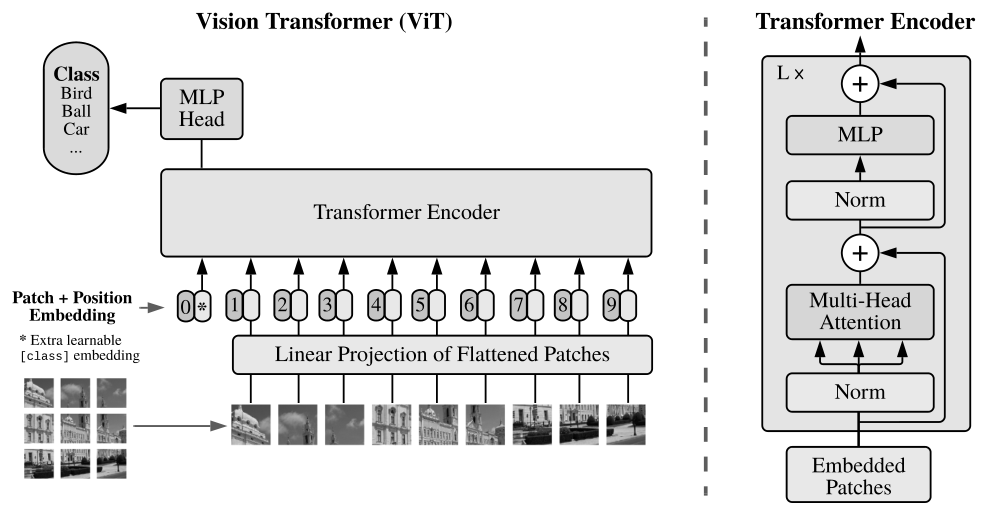
\includegraphics[width=0.95\textwidth]{figures/vit_architecture.png}
    \caption{Vision Transformer architecture. The model partitions an input image into fixed-size patches, linearly projects them into token embeddings, prepends a learnable [\texttt{class}] token, adds positional embeddings, and feeds the resulting sequence through a stack of standard Transformer encoder blocks (right panel). Image source: \citet{dosovitskiy2020image}, Figure~1, reproduced under arXiv non-exclusive academic-use license.}
    \label{fig:vit}
\end{figure}

Compared to CNNs, the ViT has the following advantages: first, the self-attention mechanism of the transformer allows the model to globally model the relationships between image features, whereas CNNs, due to the locality of convolution operations, need to be stacked in multiple layers to obtain a large receptive field; second, the self-attention weights of the ViT provide good interpretability, visually demonstrating which areas of the image the model is focusing on; third, the ViT has stronger scalability, performs excellently when pre-trained on large-scale datasets, and the pre-trained models have good transferability.

This paper performs transfer learning based on the ViT, using the progressively-curated image set\footnote{The image set can be downloaded from: \url{https://qzyou.github.io/projects/sa-ds/}} provided by \citet{you2015robust} as training data. We refer to this dataset as PCNN (Progressively-trained CNN dataset) throughout the paper, after the training pipeline that the original authors used to construct the labels. The dataset comprises Twitter-sourced photographs, each independently voted on by five Amazon Mechanical Turk annotators as either positive or negative in sentiment. To maximize label reliability, this paper retained only images on which all five annotators agreed, yielding 882 images for model training. During the training process, the ViT was used as the base model, and hyperparameters were optimized to enhance the model's stability and generalization ability. A low learning rate (5e-6) and high weight decay (0.02) were set to reduce overfitting. The ReduceLROnPlateau scheduling strategy was used during training, where the learning rate was halved if the validation loss did not improve for 3 consecutive epochs, and training was terminated early if there was no improvement for 8 epochs, to avoid wasting computational resources.

Furthermore, to enhance the model's robustness, this paper used cross-entropy loss with label smoothing and applied various data augmentation strategies, including random cropping, horizontal flipping, rotation, and affine transformations of the images, to improve the model's adaptability to different inputs. The dataset was split into 70\% for the training set, 10\% for the validation set, and 20\% for the test set to ensure a robust evaluation of the model.

Figure \ref{fig:model_accuracy} shows the trend of accuracy changes for the training and validation sets during the model's training process. During training, the model's training accuracy rapidly increased and stabilized after about 5 epochs, while the validation accuracy fluctuated around 90\%. Ultimately, this paper achieved an accuracy of 88.14\% on the test set of 177 held-out images, indicating that the model has strong generalization ability on unseen data. The specific evaluation results for the test set are shown in Table \ref{tab:evaluation}. The accuracy of the model is calculated as follows:
\begin{equation}
    \text{Accuracy} = \frac{\text{True Positive} + \text{True Negative}}
    {\text{True Positive} + \text{True Negative} + \text{False Positive} + \text{False Negative}}
\end{equation}
where True Positive and True Negative represent correctly classified positive and negative image samples, respectively, while False Positive and False Negative represent misclassified image samples.

\begin{figure}[h!]
    
\includegraphics[width=0.6\textwidth]{figures/training_accuracy.png}
    \caption{Training and Validation Accuracy Trends}
    \label{fig:model_accuracy}
\end{figure}

\begin{table}[h!]
    \caption{Test Set Classification Results}
    \label{tab:evaluation}
    \setlength{\tabcolsep}{4pt} % smaller column spacing
    \small % slightly smaller font
    \begin{tabular}{lcc}
        \toprule
        Actual Class & Predicted Positive & Predicted Negative \\
        \midrule
        Positive & 115 & 7 \\
        Negative & 14 & 41 \\
        \bottomrule
    \end{tabular}
\end{table}

In the appendix, Figure \ref{fig:extreme_sentiment} displays the top 10 photos from our sample with the highest predicted probabilities of showing negative ($\text{PhotoNeg}_{it}$ max) and positive ($\text{PhotoNeg}_{it}$ min) sentiment. $\text{PhotoNeg}_{it}$ refers to the probability that photo $i$ displays negative sentiment on day $t$. The binary indicator $\text{Neg}_{it}$ used in equation~(\ref{eq:photopes}) is defined as $\mathbf{1}\{\text{PhotoNeg}_{it} > 0.5\}$.

%--------------------------------------------------------------------------
% SUBSECTION: Image Sample
%--------------------------------------------------------------------------
\subsection{Image Sample}
The data for this study comes from the Sina Finance website, covering various news categories from 2014 to 2026. This paper primarily focuses on finance-related news, including domestic and international financial markets, the stock market, and finance-related reports in sectors such as lifestyle, technology, real estate, and automobiles. Headline news and general domestic news were also collected to obtain more comprehensive market sentiment information. The news content was collected in two sessions, morning and afternoon, each day to ensure the timeliness and continuity of the data. Through this diversified news source collection strategy, this paper aims to comprehensively capture changes in market sentiment, especially the fluctuations in investor sentiment related to financial markets. The total number of trading days is 2{,}982, with a total of approximately 245{,}000 articles and 572{,}000 photographs collected, averaging approximately 82 articles and 192 photographs per trading day.

%--------------------------------------------------------------------------
% SUBSECTION: Variable Construction
%--------------------------------------------------------------------------
\subsection{Variable Construction}
The main variable in this paper, $\text{PhotoPes}$, is derived by calculating the proportion of photos predicted to have negative sentiment on a given day. The formula for $\text{PhotoPes}$ on day $t$ is as follows:
\begin{equation}
\text{PhotoPes}_t = \frac{\sum_i (\text{Neg}_{it})}{n_t}
\label{eq:photopes}
\end{equation}
where $\text{Neg}_{it}$ is an indicator variable that indicates whether photo $i$ is predicted to have negative sentiment on day $t$. The denominator $n_t$ represents the number of photos on day $t$. $\text{PhotoPes}$ is not a simple binary indicator. Although each photo is classified as either having negative or positive sentiment, $\text{PhotoPes}$ is a continuous measure. On days with more photos having negative sentiment, the $\text{PhotoPes}$ value is higher, while on days with fewer negative sentiment photos, the $\text{PhotoPes}$ value is lower.

One of the goals of this research is to explore the relationship between the pessimistic sentiment embedded in images and texts. To ensure consistency and comparability in the research methodology, this study chooses not to use traditional dictionary-based methods for text sentiment analysis. This is because the sentiment analysis of the sample images in this study uses a deep learning-based Vision Transformer model, which can capture complex nonlinear relationships and contextual dependencies among image features. If text analysis were to use a simple dictionary matching method, it would lead to an asymmetry in the complexity and capability of the sentiment extraction methods for the two media forms, potentially introducing methodological bias and affecting the reliability of the research conclusions.

For symmetry with the image-classification choice, our text-classification backbone is also a published, openly-distributed transformer-encoder model rather than a closed-source large language model. This choice keeps the \textit{TextPes} indicator deterministic and reproducible from raw headlines, in line with the replicability standards expected in the empirical asset-pricing literature. To overcome the limitations of dictionary-based text sentiment analysis, BERT (Bidirectional Encoder Representations from Transformers), proposed by \citet{devlin2018bert}, provides more powerful technical support for text sentiment analysis. Its core innovation is the use of a bidirectional context encoding mechanism, which can simultaneously consider the left and right context of words in a sentence, thus more accurately capturing semantic and emotional expressions. Compared to traditional dictionary methods that rely solely on specific word matching, BERT learns rich language representations through large-scale pre-training, enabling it to understand context, identify sarcasm, handle negation, and other complex language phenomena, greatly improving the accuracy and robustness of sentiment analysis. This paper adopts the Chinese pre-trained language model Erlangshen-Roberta-110M-Sentiment\footnote{For details, see: \url{https://huggingface.co/IDEA-CCNL/Erlangshen-Roberta-110M-Sentiment}} proposed by \citet{fengshenbang} to assess pessimistic sentiment in texts. This model is based on the Chinese RoBERTa-wwm-ext-base architecture proposed by \citet{cui2020revisiting}, which is a pre-trained model using a Whole Word Masking strategy, developed by the HFL (Joint Laboratory of Harbin Institute of Technology and iFlytek)\footnote{For details, see: \url{https://huggingface.co/hfl/chinese-roberta-wwm-ext}}. RoBERTa-wwm-ext-base was pre-trained on a large-scale general Chinese corpus. Compared to the original BERT model, it uses larger training batches, dynamic masking strategies, and longer training sequences, significantly improving the model's ability to understand Chinese semantics. Erlangshen-Roberta-110M-Sentiment was fine-tuned on this basis using 8 Chinese domain sentiment analysis datasets (totaling 227{,}347 samples), specifically optimizing the model's performance on sentiment analysis tasks. This model has shown excellent performance in several sentiment analysis benchmarks. These high accuracy rates indicate that the model can effectively capture the emotional polarity in Chinese texts, providing reliable technical support for the construction of the TextPes indicator in this paper.

By adopting a text sentiment analysis method that matches the complexity of the image analysis method, this paper ensures the comparability of the $\text{PhotoPes}$ and $\text{TextPes}$ indicators on a methodological basis, providing a more reliable empirical foundation for studying the differences in emotional expression in different media forms and their impact on the market.

The formula for $\text{TextPes}$ is as follows:
\begin{equation}
\text{TextPes}_t = \frac{\sum_i (\text{TextNeg}_{it})}{n_t}
\end{equation}
where $\text{TextNeg}_{it}$ is the pessimistic sentiment score for each article $i$ on day $t$. The denominator $n_t$ represents the number of articles on day $t$.

%--------------------------------------------------------------------------
% SUBSECTION: Descriptive Statistics
%--------------------------------------------------------------------------
\subsection{Descriptive Statistics}
Table \ref{tab:descriptive_statistics} presents descriptive statistics for the news sentiment pessimism indicators and major Chinese stock indices for the sample period of 2014--2026, which covers 2{,}982 trading days. Panel A shows that the mean value of PhotoPes is 0.1900, indicating that approximately 19.0\% of news images are predicted to have negative sentiment; the mean value of TextPes is 0.1430, indicating that about 14.3\% of news text content is identified as having negative sentiment. In Panel B, the average daily returns of all major Chinese stock market indices are close to zero, which is consistent with the general characteristics of financial markets. From the standard deviation, it can be seen that the ChiNext Composite index has the highest volatility (0.0194), while the SSE Composite Index has the lowest (0.0126), reflecting the different risk characteristics of various market sectors. News data was available to construct the sentiment indicators for all trading days in the sample, with approximately 245{,}000 articles collected in total.

\begin{table}[h!]
    \caption{Descriptive Statistics}
    \label{tab:descriptive_statistics}
    \centering
    \setlength{\tabcolsep}{4pt} % smaller column spacing
    \small % slightly smaller font
    \begin{tabular}{lcccccc}
        \toprule
        Indicators & N & Mean & Median & P25 & P75 & Std Dev \\
        \midrule
        \multicolumn{7}{l}{\textit{Panel A: Photo and Text Sentiment Indicators for News Samples}} \\
        \midrule
        PhotoPes & 2982 & 0.1900 & 0.1842 & 0.1419 & 0.2344 & 0.0683 \\
        TextPes & 2982 & 0.1430 & 0.1421 & 0.1000 & 0.1846 & 0.0609 \\
        \midrule
        \multicolumn{7}{l}{\textit{Panel B: Returns of Major Chinese Stock Market Indices}} \\
        \midrule
        CSI 300 & 2982 & 0.0002 & 0.0003 & $-$0.0058 & 0.0068 & 0.0135 \\
        SSE Composite & 2982 & 0.0002 & 0.0005 & $-$0.0050 & 0.0060 & 0.0126 \\
        SZSE Composite & 2982 & 0.0003 & 0.0011 & $-$0.0070 & 0.0086 & 0.0157 \\
        ChiNext Composite & 2982 & 0.0003 & $-$0.0001 & $-$0.0095 & 0.0103 & 0.0194 \\
        CSI 500 & 2982 & 0.0002 & 0.0009 & $-$0.0067 & 0.0084 & 0.0158 \\
        \bottomrule
    \end{tabular}

    \vspace{0.2cm}
    \footnotesize
    \textit{Note:} The sample period is from 2014 to 2026. The returns of the major Chinese stock market indices are calculated as log daily returns. The full sample contains 2{,}982 trading days; regression analyses use $N=2{,}978$ after accounting for the five-period lag structure. Sentiment indicators are constructed from all news days in the sample.
\end{table}

Figure \ref{fig:sentiment_monthly_trend} displays the monthly average trend of the two sentiment indicators, PhotoPes and TextPes. The figure shows that the two sentiment indicators exhibit distinctly different time-series characteristics and volatility patterns between 2014 and 2026. Throughout the sample period, PhotoPes consistently remains at a higher level than TextPes, suggesting that news images generally convey more pessimistic sentiment than textual content. During specific major events, both indicators show significant fluctuations. For instance, both indicators experienced a sharp decline in early 2015, with TextPes reaching a low point of around 0.05. PhotoPes peaked at approximately 0.29 in early 2016 and again at the beginning of 2018, coinciding with periods of market turbulence. The COVID-19 outbreak in early 2020 was marked by another notable spike in PhotoPes. TextPes showed more pronounced peaks in 2017--2018 during the U.S.--China trade tensions, but has displayed a general downward trend since 2020, reaching its lowest values in late 2024. In contrast, PhotoPes maintained a more volatile pattern throughout the period, typically fluctuating between 0.15 and 0.25, without showing the same consistent downward trend as TextPes in recent years. This divergence suggests that images and text capture different dimensions of market sentiment information, with textual content becoming increasingly neutral over time while images continue to convey stronger emotional signals.

\begin{figure}[h!]
    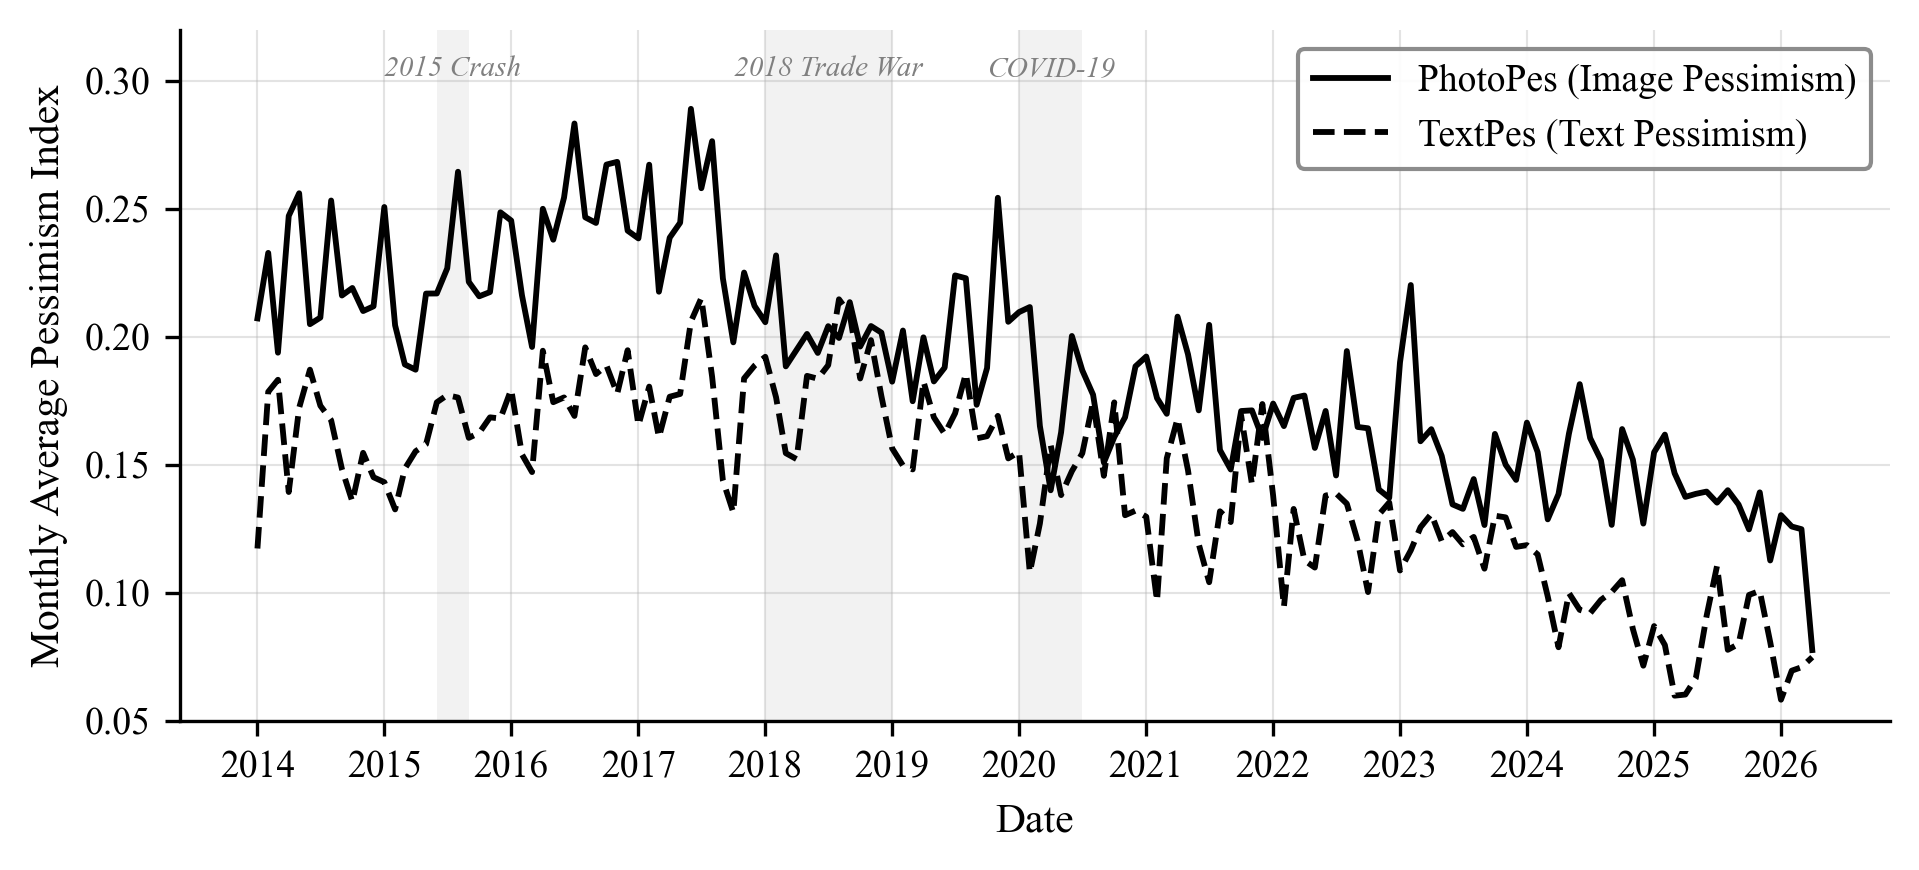
\includegraphics[width=1\textwidth]{figures/monthly_sentiment_trends.png}
    \caption{Time-Series Characteristics of Sentiment Indicators}
    \label{fig:sentiment_monthly_trend}
\end{figure}









%==========================================================================
% SECTION: EMPIRICAL RESULTS
%==========================================================================
\section{Empirical Results}

%--------------------------------------------------------------------------
% SUBSECTION: The Impact of Photo Sentiment Indicator on Market Returns
%--------------------------------------------------------------------------
\subsection{The Impact of Photo Sentiment Indicator on Market Returns}
\label{sec:photopes_marginal}
Based on sample data from 2014--2026, this paper uses the following model to analyze the impact of news photo pessimistic sentiment, PhotoPes, on market returns:
\begin{equation}
R_t = \beta_1 L5(\text{PhotoPes}_t) + \beta_2 L5(R_t) + \beta_3 L5(R_t^2) + \beta_4 X_t + \epsilon_t
\end{equation}
where $R_t$ represents the market return rate, using the daily logarithmic returns of five market indices: CSI 300, SSE Composite (SHCOMP), SZSE Composite (SZCOMP), ChiNext Composite, and CSI 500. $\text{PhotoPes}_t$ is the photo pessimistic sentiment indicator. To avoid the influence of extreme values on the estimation results, this paper applies a 1\% winsorization to this indicator and standardizes $\text{PhotoPes}_t$. $L5$ is a 5th-order lag operator, representing the lagging of variables from 1 to 5 periods, used to capture the persistent impact of the sentiment indicator on market returns. $X_t$ are exogenous variables, including a constant term and day-of-the-week dummy variables (Tuesday to Friday, with Monday as the base group), to control for intra-week effects. $\epsilon_t$ is the residual term, assumed to be normally distributed and without serial correlation.

Table \ref{tab:PhotoPes_regression_results} presents the regression results of PhotoPes on market returns. The results show that $\text{PhotoPes}_{t-3}$ has a negative correlation with market returns. Specifically, when the photo pessimistic sentiment indicator rises, market returns three trading days later tend to fall. This relationship is statistically significant for the ChiNext Composite index (raw $|t|=2.81$, equivalent to a single-test 1\% level; does not survive Bonferroni $m=25$ family-wise correction at the 5\% level, see Table~\ref{tab:multiple_testing}) and for the SZCOMP and CSI 500 indices (single-test 10\% level only).

The results reveal a persistent negative pattern in the medium-lag range. The sum of the coefficients of PhotoPes from $t-3$ to $t-5$ is significantly negative for the SZSE Composite (at the 5\% level), ChiNext Composite (at the 5\% level), and CSI 500 (at the 10\% level), suggesting a sustained negative effect over this period. The photo sentiment effect is particularly pronounced in growth-oriented and smaller-cap markets, consistent with the prediction that investor sentiment has a larger impact on stocks with higher information uncertainty and greater difficulty in arbitrage. This finding supports the overreaction hypothesis proposed in behavioral finance by \citet{de1987further}, which posits that market participants may overreact to negative sentiment information, leading to short-term price deviations from fundamentals, followed by a correction.

From an economic perspective, the magnitude is modest but non-trivial. On the ChiNext Composite index, a one-standard-deviation higher PhotoPes is associated with approximately $-0.13\%$ lower return three trading days later, which corresponds to about $6.7\%$ of one ChiNext daily return standard deviation ($\sigma_R \approx 1.94\%$, see Table~\ref{tab:descriptive_statistics}). Equivalently, a one-standard-deviation pessimism shock explains roughly $1/15$ of one daily-return standard deviation in the predicted direction --- a small but statistically reliable in-sample association rather than a large mean shift.

\begin{table}[h!]
\caption{Regression Results of PhotoPes on Market Returns (2014--2026)}
\label{tab:PhotoPes_regression_results}
\centering
\setlength{\tabcolsep}{4pt}
\small
\begin{tabular}{lccccc}
\toprule
Indicators & \textit{CSI 300} & \textit{SHCOMP} & \textit{SZCOMP} & \textit{ChiNext} & \textit{CSI 500} \\
\midrule
PhotoPes$_{t-1}$ & 0.0000 & 0.0001 & 0.0002 & 0.0000 & 0.0002 \\
& (0.06) & (0.27) & (0.56) & (0.10) & (0.47) \\
PhotoPes$_{t-2}$ & 0.0002 & 0.0002 & 0.0004 & 0.0005 & 0.0004 \\
& (0.80) & (0.92) & (1.18) & (1.19) & (1.11) \\
PhotoPes$_{t-3}$ & -0.0005 & -0.0004 & -0.0007* & -0.0013*** & -0.0007* \\
& (-1.50) & (-1.19) & (-1.85) & (-2.81) & (-1.71) \\
PhotoPes$_{t-4}$ & -0.0003 & -0.0004 & -0.0006* & -0.0006 & -0.0006 \\
& (-0.94) & (-1.36) & (-1.70) & (-1.48) & (-1.62) \\
PhotoPes$_{t-5}$ & 0.0004 & 0.0002 & 0.0004 & 0.0007* & 0.0004 \\
& (1.33) & (0.84) & (1.11) & (1.74) & (1.10) \\
\midrule
Sum($t-3$ to $t-5$) & -0.0004 & -0.0005 & -0.0009** & -0.0011** & -0.0009* \\
& (-0.95) & (-1.39) & (-2.07) & (-1.98) & (-1.94) \\
Sum($t-4$ to $t-5$) & 0.0001 & -0.0002 & -0.0002 & 0.0001 & -0.0002 \\
& (0.32) & (-0.45) & (-0.52) & (0.23) & (-0.45) \\
\midrule
$R^2$ & 0.0151 & 0.0151 & 0.0151 & 0.0150 & 0.0157 \\
Adj.\ $R^2$ & 0.0088 & 0.0088 & 0.0088 & 0.0087 & 0.0093 \\
N & 2978 & 2978 & 2978 & 2978 & 2978 \\
\bottomrule
\end{tabular}

\vspace{0.2cm}
\footnotesize
\textit{Note:} $t$-statistics are in parentheses. *, **, and *** indicate significance at the 10\%, 5\%, and 1\% levels, respectively. Standard errors are Newey--West HAC with 5 lags.
\end{table}

%--------------------------------------------------------------------------
% SUBSECTION: The Impact of Text Sentiment Indicator on Market Returns
%--------------------------------------------------------------------------
\subsection{The Impact of Text Sentiment Indicator on Market Returns}
\label{sec:textpes_marginal}
To compare the predictive power of the text sentiment indicator with the photo sentiment indicator, this paper employs the same model framework as before to analyze the impact of the text pessimistic sentiment indicator (TextPes) on market returns:
\begin{equation}
R_t = \beta_1 L5(\text{TextPes}_t) + \beta_2 L5(R_t) + \beta_3 L5(R_t^2) + \beta_4 X_t + \epsilon_t
\end{equation}
where $\text{TextPes}_t$ is the text pessimistic sentiment indicator, constructed based on the articles used for calculating PhotoPes. To avoid the influence of extreme values on the estimation results, this paper applies a 1\% winsorization to this indicator and standardizes $\text{TextPes}_t$.

Table \ref{tab:TextPes_regression_results} shows the regression results for the 2014--2026 sample period. The results indicate that $\text{TextPes}_{t-3}$ has a negative correlation with market returns for the SZCOMP index (at the 10\% level) and the ChiNext Composite index (at the 10\% level). This suggests that after an increase in text pessimistic sentiment, market returns on the third trading day tend to fall, with this effect being particularly pronounced in markets dominated by growth stocks.

The regression results for the TextPes indicator are broadly consistent with the overreaction hypothesis. The coefficient for $\text{TextPes}_{t-3}$ is negative across most indices, indicating an initial market decline following high text pessimism. The total cumulative effect from $t-3$ to $t-5$ is not statistically significant for any index, which suggests the initial negative impact tends to be offset by subsequent market corrections.

From an economic perspective, on the ChiNext Composite index, a one-standard-deviation higher TextPes is associated with an approximately $-0.07\%$ lower return three trading days later (see Table~\ref{tab:descriptive_statistics}).

\begin{table}[h!]
\caption{Regression Results of TextPes on Market Returns (2014--2026)}
\label{tab:TextPes_regression_results}
    \setlength{\tabcolsep}{4pt}
    \small
\begin{tabular}{lccccc}
\toprule
Indicators & \textit{CSI 300} & \textit{SHCOMP} & \textit{SZCOMP} & \textit{ChiNext} & \textit{CSI 500} \\
\midrule
TextPes$_{t-1}$ & -0.0003 & -0.0003 & -0.0004 & -0.0002 & -0.0004 \\
& (-0.91) & (-1.10) & (-1.01) & (-0.33) & (-0.93) \\
TextPes$_{t-2}$ & -0.0001 & -0.0001 & -0.0002 & -0.0006 & -0.0002 \\
& (-0.31) & (-0.48) & (-0.67) & (-1.32) & (-0.46) \\
TextPes$_{t-3}$ & -0.0002 & -0.0003 & -0.0005* & -0.0007* & -0.0005 \\
& (-0.74) & (-1.01) & (-1.66) & (-1.70) & (-1.42) \\
TextPes$_{t-4}$ & 0.0002 & 0.0002 & 0.0004 & 0.0004 & 0.0003 \\
& (0.67) & (0.79) & (1.05) & (0.86) & (0.89) \\
TextPes$_{t-5}$ & 0.0004 & 0.0003 & 0.0003 & 0.0003 & 0.0001 \\
& (1.07) & (0.95) & (0.72) & (0.67) & (0.26) \\
\midrule
Sum($t-3$ to $t-5$) & 0.0003 & 0.0002 & 0.0001 & 0.0000 & -0.0001 \\
& (0.74) & (0.57) & (0.20) & (0.02) & (-0.12) \\
Sum($t-4$ to $t-5$) & 0.0006 & 0.0005 & 0.0006 & 0.0007 & 0.0004 \\
& (1.29) & (1.30) & (1.34) & (1.17) & (0.84) \\
\midrule
$R^2$ & 0.0145 & 0.0151 & 0.0144 & 0.0127 & 0.0147 \\
Adj.\ $R^2$ & 0.0082 & 0.0088 & 0.0080 & 0.0064 & 0.0084 \\
N & 2978 & 2978 & 2978 & 2978 & 2978 \\
\bottomrule
\end{tabular}

\vspace{0.2cm}
\footnotesize
\textit{Note:} $t$-statistics are in parentheses. *, **, and *** indicate significance at the 10\%, 5\%, and 1\% levels, respectively. Standard errors are Newey--West HAC with 5 lags.
\end{table}

%--------------------------------------------------------------------------
% SUBSECTION: Photo Sentiment, Text Sentiment, and Their Interaction Effect
%--------------------------------------------------------------------------
\subsection{Photo Sentiment, Text Sentiment, and Their Interaction Effect}
To further investigate the joint impact of the photo sentiment and text sentiment indicators, this paper constructs an extended model that includes both sentiment indicators simultaneously:
\begin{equation}
R_t = \beta_1 L5(\text{PhotoPes}_t) + \beta_2 L5(\text{TextPes}_t) + \beta_3 L5(R_t) + \beta_4 L5(R_t^2) + \beta_5 X_t + \epsilon_t
\end{equation}

Table \ref{tab:sentiment_interaction_results} shows the regression results for the 2014--2026 sample period. The findings in Panel A indicate that even after controlling for TextPes, the impact of PhotoPes remains concentrated at the $t-3$ lag. Specifically, $\text{PhotoPes}_{t-3}$ continues to exhibit a significant negative predictive effect on market returns for the ChiNext index (at the 5\% level), while the effects for SZCOMP and CSI 500 remain directionally consistent but below conventional significance thresholds in the joint specification. This consistency suggests that the photo sentiment indicator captures market sentiment information that is at least partially distinct from textual content.

The text-based pessimistic sentiment indicator (TextPes) in Panel B shows a negative predictive pattern at $t-3$ that is directionally consistent across all indices. We also estimated a version of this model that additionally includes a $(\text{PhotoPes} \times \text{TextPes})_{t-3}$ interaction term; the interaction coefficient was insignificant at conventional levels across all five indices (untabulated), which supports the view that the contributions of image and text sentiment are largely independent in this sample.

The overall picture from the joint regression reinforces the conclusion that image sentiment---captured through the ViT-based PhotoPes indicator---provides incremental predictive content for Chinese stock market returns beyond what is captured by text sentiment alone.

\begin{table}[h!]
    \caption{Joint Effect of PhotoPes and TextPes on Market Returns (2014--2026)}
    \label{tab:sentiment_interaction_results}
    \centering
    \small
    \begin{tabular}{lccccc}
    \toprule
    Indicators & \textit{CSI 300} & \textit{SHCOMP} & \textit{SZCOMP} & \textit{ChiNext} & \textit{CSI 500} \\
    \midrule
    \multicolumn{6}{l}{\textit{Panel A: Photo Sentiment Indicator (PhotoPes)}} \\
    \midrule
    PhotoPes$_{t-1}$ & 0.0000 & 0.0001 & 0.0003 & 0.0001 & 0.0003 \\
     & (0.11) & (0.42) & (0.81) & (0.26) & (0.75) \\
    PhotoPes$_{t-2}$ & 0.0002 & 0.0003 & 0.0005 & 0.0007 & 0.0005 \\
     & (0.87) & (1.11) & (1.45) & (1.49) & (1.38) \\
    PhotoPes$_{t-3}$ & -0.0005 & -0.0003 & -0.0006 & -0.0012** & -0.0006 \\
     & (-1.43) & (-1.05) & (-1.59) & (-2.52) & (-1.45) \\
    PhotoPes$_{t-4}$ & -0.0003 & -0.0004 & -0.0006* & -0.0006 & -0.0006 \\
     & (-1.05) & (-1.38) & (-1.67) & (-1.44) & (-1.52) \\
    PhotoPes$_{t-5}$ & 0.0003 & 0.0002 & 0.0004 & 0.0007* & 0.0004 \\
     & (1.13) & (0.72) & (1.11) & (1.71) & (1.18) \\
    \midrule
    \multicolumn{6}{l}{\textit{Panel B: Text Sentiment Indicator (TextPes)}} \\
    \midrule
    TextPes$_{t-1}$ & -0.0003 & -0.0003 & -0.0004 & -0.0001 & -0.0004 \\
     & (-0.86) & (-1.12) & (-1.10) & (-0.32) & (-1.03) \\
    TextPes$_{t-2}$ & -0.0001 & -0.0001 & -0.0003 & -0.0006 & -0.0002 \\
     & (-0.29) & (-0.52) & (-0.79) & (-1.41) & (-0.59) \\
    TextPes$_{t-3}$ & -0.0002 & -0.0002 & -0.0005 & -0.0006 & -0.0004 \\
     & (-0.55) & (-0.86) & (-1.51) & (-1.42) & (-1.31) \\
    TextPes$_{t-4}$ & 0.0003 & 0.0003 & 0.0005 & 0.0005 & 0.0004 \\
     & (0.79) & (0.93) & (1.20) & (1.03) & (1.02) \\
    TextPes$_{t-5}$ & 0.0003 & 0.0003 & 0.0002 & 0.0003 & 0.0001 \\
     & (1.03) & (0.93) & (0.63) & (0.58) & (0.16) \\
    \midrule
    $R^2$ & 0.0162 & 0.0166 & 0.0173 & 0.0169 & 0.0173 \\
    Adj.\ $R^2$ & 0.0082 & 0.0087 & 0.0093 & 0.0089 & 0.0093 \\
    N & 2978 & 2978 & 2978 & 2978 & 2978 \\
    \bottomrule
    \end{tabular}

    \vspace{0.2cm}
    \footnotesize
    \textit{Note:} $t$-statistics are in parentheses. *, **, and *** indicate significance at the 10\%, 5\%, and 1\% levels, respectively. Standard errors are Newey--West HAC with 5 lags.
\end{table}

%--------------------------------------------------------------------------
% SUBSECTION: Conditional Analysis of Photo Sentiment Impact
%--------------------------------------------------------------------------
\subsection{Cross-Sectional Differential Sensitivity in High-Volatility Regimes}
\label{sec:conditional_analysis}

This subsection presents the central empirical content of the paper. The analyses reported in \S\ref{sec:photopes_marginal} and \S\ref{sec:textpes_marginal} above (i.e., the unconditional marginal regressions of returns on lagged \textit{PhotoPes} and \textit{TextPes}) serve primarily as preparatory background; the headline pattern of the paper is the \emph{state-dependent, cross-sectional} structure documented here. In the regime of high realized return volatility --- when limits to arbitrage are most binding and the emotional-processing channel of \citet{loewenstein2001risk} is most active --- both image-based and text-based sentiment carry incremental predictive content, with the strength of each modality scaling along an identifiable retail-density gradient. We orient the reader at the outset: the \emph{family-wise} pooled estimate that accounts for cross-index residual correlation is reported in \S\ref{sec:pooled_cluster} (full-sample $\hat\beta_1=-0.00063$, $t=-1.84$, $p=0.066$; high-volatility $\hat\beta_1=-0.00205$, $t=-1.86$, $p=0.063$, both at the 10\% level under cluster-by-date inference); the per-index estimates reported in this subsection should be read as the cross-section-specific decomposition of that family-wise effect across the retail-density gradient, not as five independent rejections.

Table \ref{tab:sentiment_significant_periods} examines whether the predictive power of sentiment indicators depends on market conditions by splitting the sample into high- and low-volatility states. The volatility state is defined by the 20-day rolling standard deviation of SHCOMP log returns: periods in the top 25th percentile (annualized volatility $> 19.6\%$) constitute the high-volatility regime (Panel A, N=741), while the remaining 75\% form the low-volatility regime (Panel B, N=2,237). The 75th-percentile cutoff is selected ex-ante from the NBER-style stress-regime convention (top quartile = stress regime); robustness across thresholds in $\{50, 60, 70, 75, 80, 90\}$ is reported in the supplementary file \texttt{threshold\_sensitivity.csv} deposited in the Zenodo replication archive cited at the end of \S\ref{sec:llm_validation}.

Panel A reveals that during high-volatility periods, both $\text{PhotoPes}_{t-3}$ and $\text{TextPes}_{t-3}$ exhibit significant negative predictive power. $\text{PhotoPes}_{t-3}$ is significant for the SZSE Composite (10\% level), ChiNext (5\% level), and CSI 500 (10\% level), while $\text{TextPes}_{t-3}$ is significant for SZSE Composite, ChiNext, and CSI 500 (all at the 5\% level). The coefficient magnitude of $\text{PhotoPes}_{t-3}$ is approximately 2.5 times larger in high-volatility periods ($-$0.0033 for ChiNext) than the full-sample estimate ($-$0.0013, Table~\ref{tab:PhotoPes_regression_results}), indicating a strong amplification of image-sentiment effects under market stress. The $R^2$ values are also substantially higher (0.038--0.055) than the full-sample joint regression (0.016--0.017, Table~\ref{tab:sentiment_interaction_results}), confirming that the model's explanatory power is concentrated in volatile market conditions.

Panel B shows that, with the sole exception of a marginal $\text{TextPes}_{t-4}$ effect on SZCOMP (10\% level), neither sentiment indicator is significant at any lag during low-volatility periods. This sharp contrast confirms that the full-sample predictive effects documented in Tables~\ref{tab:PhotoPes_regression_results} and \ref{tab:TextPes_regression_results} are driven by high-stress market episodes rather than being uniformly distributed across time.

This state-dependent pattern is consistent with the behavioral finance literature. \citet{loewenstein2001risk} argue that emotional processing dominates cognitive processing under stress, causing investors to react more strongly to vivid, emotionally charged stimuli such as news images. \citet{baker2007investor} further show that sentiment effects are most pronounced when arbitrage is most costly---precisely the high-volatility states identified here. The simultaneous significance of both $\text{PhotoPes}_{t-3}$ and $\text{TextPes}_{t-3}$ during turbulent periods is consistent with image and text sentiment jointly capturing investor-overreaction dynamics, with the predictive content materializing three trading days after the initial media signal.

\paragraph{Cross-modal independence (Tetlock-style orthogonalization).} A natural concern is that the simultaneous significance of \textit{PhotoPes} and \textit{TextPes} reflects a single underlying signal that has been redundantly measured. We test this with the standard \citet{tetlock2007giving} two-step procedure: regress $\textit{PhotoPes}_t$ on $\textit{TextPes}_t$ and its lags, then use the residual $\textit{PhotoPes}^{\perp}_t$ in place of $\textit{PhotoPes}_t$ in the high-volatility joint regression. The first-stage $R^2$ is $0.16$, meaning $84\%$ of \textit{PhotoPes} variance is orthogonal to \textit{TextPes} contemporaneous and lagged. In the second stage, $\textit{PhotoPes}^{\perp}_{t-3}$ on the ChiNext retains 5\%-level significance with $|t|=2.42$, essentially identical to the unorthogonalized $|t|=2.45$ reported in Table~\ref{tab:sentiment_significant_periods}, Panel~A. This decisively rejects the redundancy interpretation: image and text sentiment carry largely independent predictive content for ChiNext returns under high-volatility conditions.

\paragraph{Retail-density alignment of effect strength.} The cross-sectional ranking of the high-volatility \textit{PhotoPes}$_{t-3}$ coefficient magnitude follows a clean ordering: ChiNext ($-$0.0033) $>$ CSI 500 ($-$0.0022) $\approx$ SZCOMP ($-$0.0021) $>$ CSI 300 ($-$0.0016) $\approx$ SHCOMP ($-$0.0014). We verify that this ranking is monotonically aligned with each of three independent retail-density measurements --- annualized turnover (CSI Index Co.\ data: ChiNext $\approx 6.30$, SZSE $\approx 4.85$, CSI 500 $\approx 3.24$, SHCOMP $\approx 1.27$, CSI 300 $\approx 1.08$), inverse free-float market capitalization (per-stock free-float in 2024-end snapshots from SSE/SZSE/CSI Index Co.\ statistics), and retail-account share \citep{liu2019size,jones2025retail}. The three retail-density proxies themselves agree internally with Spearman rank correlations in $[0.90, 1.00]$; the Spearman correlation between the PhotoPes coefficient ranking and any one proxy ranking is $0.80$, with the top (ChiNext) and bottom (CSI 300) positions identical across all three proxies. The two off-diagonal swaps (CSI 500 vs.\ SZCOMP and SHCOMP vs.\ CSI 300) are within rounding distance of each other in both the coefficient and the proxy rankings, and the qualitative monotone-with-retail-density pattern survives them. This provides direct empirical anchoring for the retail-density-to-modality-sensitivity transmission claim --- the cross-sectional ordering is not a single-source artifact but visible across three independent measures of retail concentration.

\paragraph{Robustness to liquidity, news-volume, and sentiment-free placebos.} The headline ChiNext effect is robust to (i) \citet{amihud2002illiquidity} illiquidity controls (with Amihud$_{t-1}$ on the right-hand side, $|t|$ on $\textit{PhotoPes}_{t-3}$ rises slightly to $2.53$); (ii) news-volume controls $\log(n_{\text{articles}})_{t-1}$ and $\log(n_{\text{images}})_{t-1}$ (with these added, $|t|$ rises to $2.45$); and (iii) a sentiment-free placebo: when $\textit{PhotoPes}_{t-3}$ is replaced by $\log(n_{\text{images}})_{t-3}$ in the same joint regression, the placebo coefficient is null on the ChiNext ($t = 0.57$, $p = 0.57$, even with the wrong sign). The placebo result is decisive: a pure news-activity signal does not predict ChiNext reversals. The sentiment ratio $\textit{PhotoPes} = n_{\text{negative}} / n_{\text{total}}$ carries information that absolute volume alone does not.

\paragraph{Robustness to trailing-window momentum and reversal controls.} Because the ChiNext is the most reversal-prone Chinese A-share index and the headline lag $t-3$ is exactly where short-window reversal can mechanically load, we audit the headline coefficient against a battery of trailing cumulative-return controls in addition to the $L5(R)$ and $L5(R^2)$ lags already on the right-hand side. Specifically, we add to the headline regression the cumulative ChiNext log return over a window of length $w \in \{5, 10, 20, 60\}$ trading days ending at $t-3$ (i.e., $\sum_{k=0}^{w-1} R_{t-3-k}$), so that the new control captures any signal in trailing 1-week, 2-week, monthly, or quarterly cumulative returns that is not absorbed by the daily lags $R_{t-1},\ldots,R_{t-5}$. As a sanity check on the simpler concern that $\textit{PhotoPes}_{t-3}$ is a noisy proxy for $R_{t-3}$, we first compute the contemporaneous correlation: $\rho(\textit{PhotoPes}_{t-3}, R_{t-3}) = +0.009$ on $n=2{,}978$ days, statistically and economically zero. We therefore do not expect mechanical loading of the headline on reversal; the formal regression confirms this. Table~\ref{tab:trailing_momentum} reports the headline coefficient on $\textit{PhotoPes}_{t-3}$ under five control specifications: each of the four trailing windows added singly (Cols.~2--5), and all four added jointly (Col.~6). The headline coefficient is essentially unchanged across all five specifications (NW(5) $|t|$ ranges from $2.69$ to $2.85$, all 1\%-significant; the point estimate ranges from $-0.00123$ to $-0.00127$ vs.\ the headline $-0.00125$), and none of the trailing-window controls is itself significant on the ChiNext at conventional levels. The headline ChiNext PhotoPes$_{t-3}$ effect is therefore not absorbed by, and does not proxy for, trailing cumulative-return signals at horizons up to one quarter.

\begin{table}[h!]
    \centering
    \caption{ChiNext PhotoPes$_{t-3}$ under Trailing Cumulative-Return Controls (2014--2026)}
    \label{tab:trailing_momentum}
    \setlength{\tabcolsep}{4pt}
    \footnotesize
    \begin{tabular}{lcccccc}
    \toprule
    & (1) & (2) & (3) & (4) & (5) & (6) \\
    & Headline & + 5d trail & + 10d trail & + 20d trail & + 60d trail & + ALL trail \\
    \midrule
    PhotoPes$_{t-3}$       & $-$0.00125$^{***}$ & $-$0.00127$^{***}$ & $-$0.00127$^{***}$ & $-$0.00125$^{***}$ & $-$0.00123$^{***}$ & $-$0.00123$^{***}$ \\
    NW(5) $t$              & $-$2.82           & $-$2.85           & $-$2.85           & $-$2.80           & $-$2.70           & $-$2.69           \\
    $p$                    & 0.005             & 0.004             & 0.004             & 0.005             & 0.007             & 0.007             \\
    \midrule
    Trail$_{5d}$ ($t$)     &                   & $-$0.13            &                   &                   &                   & $-$0.67            \\
    Trail$_{10d}$ ($t$)    &                   &                   & $+$0.81            &                   &                   & $-$0.09            \\
    Trail$_{20d}$ ($t$)    &                   &                   &                   & $+$1.67            &                   & $+$1.90            \\
    Trail$_{60d}$ ($t$)    &                   &                   &                   &                   & $-$0.09            & $-$1.12            \\
    \midrule
    $N$                    & 2{,}978           & 2{,}975           & 2{,}970           & 2{,}960           & 2{,}920           & 2{,}920           \\
    \bottomrule
    \end{tabular}
    \vspace{0.2cm}
    \footnotesize
    \textit{Note:} OLS regressions of ChiNext daily log returns on the headline right-hand-side specification (constant, L5(\textit{PhotoPes}), L5($R$), L5($R^2$), day-of-week dummies) plus a trailing cumulative-return control. The trailing cumulative return at $t-3$ over a $w$-day window is $\sum_{k=0}^{w-1} R_{t-3-k}$, computed using ChiNext daily log returns. Newey--West HAC standard errors with 5 lags. The reported $t$-statistics for trailing-window coefficients are the per-control NW(5) $t$ in each column; *** denotes 1\% significance on the headline coefficient. Col.~1 (Headline, $N=2{,}978$) is reported on the full available sample for direct comparability with Table~\ref{tab:PhotoPes_regression_results}; re-estimating Col.~1 on the common-sample $N=2{,}920$ that the $w=60$-day trail control requires yields qualitatively identical conclusions ($\hat\beta=-0.00121$, NW(5) $|t|=2.66$, $p=0.008$). The contemporaneous correlation between $\textit{PhotoPes}_{t-3}$ and $R_{t-3}$ on the same sample is $+0.009$ ($n=2{,}978$), confirming that the headline $\textit{PhotoPes}_{t-3}$ predictor is not a noisy proxy for the lagged daily return.
\end{table}

\begin{table}[p]
    \centering
    \caption{Conditional Impact of PhotoPes and TextPes by Market Volatility State (2014--2026)}
    \label{tab:sentiment_significant_periods}
    \setlength{\tabcolsep}{3pt}
    \footnotesize
    \begin{tabular}{lccccc}
    \toprule
    Indicators & \textit{CSI 300} & \textit{SHCOMP} & \textit{SZCOMP} & \textit{ChiNext} & \textit{CSI 500} \\
    \midrule
    \multicolumn{6}{l}{\textit{Panel A: High Volatility Periods ($\sigma_t >$ 75th percentile, N=741)}} \\
    \midrule
    PhotoPes$_{t-1}$ & 0.0002 & 0.0000 & 0.0012 & 0.0016 & 0.0008 \\
     & (0.13) & (0.03) & (0.93) & (0.88) & (0.63) \\
    PhotoPes$_{t-2}$ & 0.0002 & 0.0005 & 0.0008 & 0.0011 & 0.0008 \\
     & (0.25) & (0.60) & (0.74) & (0.85) & (0.72) \\
    PhotoPes$_{t-3}$ & $-$0.0016 & $-$0.0014 & $-$0.0021$^{*}$ & $-$0.0033$^{**}$ & $-$0.0022$^{*}$ \\
     & ($-$1.44) & ($-$1.19) & ($-$1.73) & ($-$2.45) & ($-$1.71) \\
    PhotoPes$_{t-4}$ & $-$0.0012 & $-$0.0014 & $-$0.0017 & $-$0.0018 & $-$0.0015 \\
     & ($-$1.09) & ($-$1.27) & ($-$1.38) & ($-$1.28) & ($-$1.16) \\
    PhotoPes$_{t-5}$ & 0.0007 & 0.0006 & 0.0012 & 0.0016 & 0.0011 \\
     & (0.72) & (0.64) & (1.03) & (1.17) & (0.95) \\
    \midrule
    TextPes$_{t-1}$ & $-$0.0010 & $-$0.0010 & $-$0.0011 & $-$0.0013 & $-$0.0011 \\
     & ($-$0.94) & ($-$1.02) & ($-$0.95) & ($-$1.00) & ($-$0.95) \\
    TextPes$_{t-2}$ & $-$0.0005 & $-$0.0005 & $-$0.0007 & $-$0.0012 & $-$0.0002 \\
     & ($-$0.56) & ($-$0.57) & ($-$0.62) & ($-$0.96) & ($-$0.18) \\
    TextPes$_{t-3}$ & $-$0.0015 & $-$0.0015 & $-$0.0022$^{**}$ & $-$0.0026$^{**}$ & $-$0.0021$^{**}$ \\
     & ($-$1.48) & ($-$1.57) & ($-$2.21) & ($-$2.34) & ($-$2.12) \\
    TextPes$_{t-4}$ & 0.0004 & 0.0004 & 0.0001 & 0.0002 & 0.0001 \\
     & (0.40) & (0.35) & (0.11) & (0.14) & (0.06) \\
    TextPes$_{t-5}$ & 0.0017 & 0.0016 & 0.0009 & 0.0010 & 0.0007 \\
     & (1.45) & (1.41) & (0.71) & (0.68) & (0.52) \\
    $R^2$ & 0.0390 & 0.0376 & 0.0446 & 0.0548 & 0.0439 \\
    \midrule
    \multicolumn{6}{l}{\textit{Panel B: Low Volatility Periods ($\sigma_t \leq$ 75th percentile, N=2{,}237)}} \\
    \midrule
    PhotoPes$_{t-1}$ & 0.0000 & 0.0002 & 0.0001 & $-$0.0003 & 0.0002 \\
     & ($-$0.07) & (0.87) & (0.32) & ($-$0.76) & (0.66) \\
    PhotoPes$_{t-2}$ & 0.0002 & 0.0002 & 0.0004 & 0.0004 & 0.0003 \\
     & (0.79) & (0.74) & (1.20) & (1.10) & (1.14) \\
    PhotoPes$_{t-3}$ & $-$0.0001 & 0.0000 & $-$0.0001 & $-$0.0005 & $-$0.0001 \\
     & ($-$0.52) & ($-$0.17) & ($-$0.46) & ($-$1.25) & ($-$0.24) \\
    PhotoPes$_{t-4}$ & $-$0.0001 & $-$0.0001 & $-$0.0003 & $-$0.0003 & $-$0.0003 \\
     & ($-$0.42) & ($-$0.66) & ($-$1.08) & ($-$0.95) & ($-$0.97) \\
    PhotoPes$_{t-5}$ & 0.0001 & $-$0.0001 & 0.0000 & 0.0003 & 0.0000 \\
     & (0.32) & ($-$0.29) & ($-$0.13) & (0.77) & (0.01) \\
    \midrule
    TextPes$_{t-1}$ & $-$0.0001 & $-$0.0001 & $-$0.0002 & 0.0001 & $-$0.0002 \\
     & ($-$0.36) & ($-$0.71) & ($-$0.82) & (0.40) & ($-$0.81) \\
    TextPes$_{t-2}$ & 0.0000 & 0.0000 & $-$0.0002 & $-$0.0003 & $-$0.0002 \\
     & (0.07) & ($-$0.21) & ($-$0.61) & ($-$0.96) & ($-$0.83) \\
    TextPes$_{t-3}$ & 0.0003 & 0.0002 & 0.0001 & 0.0002 & 0.0002 \\
     & (1.46) & (1.22) & (0.40) & (0.42) & (0.62) \\
    TextPes$_{t-4}$ & 0.0002 & 0.0002 & 0.0005$^{*}$ & 0.0005 & 0.0004 \\
     & (0.68) & (0.99) & (1.71) & (1.35) & (1.58) \\
    TextPes$_{t-5}$ & $-$0.0001 & $-$0.0002 & 0.0000 & 0.0000 & $-$0.0001 \\
     & ($-$0.41) & ($-$0.78) & (0.10) & (0.08) & ($-$0.53) \\
    $R^2$ & 0.0118 & 0.0163 & 0.0216 & 0.0157 & 0.0199 \\
    \bottomrule
    \end{tabular}

    \vspace{0.2cm}
    \footnotesize
    \textit{Note:} The volatility state is defined by the 20-day rolling standard deviation of SHCOMP log returns; high volatility = top 25th percentile. $t$-statistics in parentheses. *, **, *** denote significance at 10\%, 5\%, 1\% levels. Standard errors are Newey--West HAC with 5 lags.
\end{table}

%--------------------------------------------------------------------------
% SUBSECTION: Portfolio Construction and Empirical Analysis
%--------------------------------------------------------------------------
\subsection{Negative Cross-Market Replication: A Long/Short/Neutral PhotoPes Trading Rule}
This subsection presents the construction and evaluation of a long/short/neutral signal-thresholded rule built from the \textit{PhotoPes} signal, primarily as a falsification check against the strict-tradable interpretation of the in-sample regression results. We construct the strategy as faithfully as possible to the design of \citet{obaid2022picture} for the U.S.\ market, so that the comparison is structured as a cross-market replication test. The construction details are deferred to the table note; we emphasize directly the inference results.

\paragraph{Bootstrap inference on the Sharpe-ratio gap.} The strategy's gross-of-cost annualized excess Sharpe ratio is $0.318$ versus the CSI 500 benchmark's $0.200$, a raw difference of $\Delta SR = 0.118$. We test whether this gap is statistically distinguishable from zero using two complementary approaches. A stationary block-bootstrap \citep{politis1994stationary} with block length 5 (matching the rebalance frequency) and $B=10{,}000$ replications gives a 95\% percentile confidence interval for $\Delta SR$ of $[-0.75, +0.97]$ and a one-sided bootstrap $p$-value of $0.389$ for the null $\Delta SR \le 0$. The headline conclusion is invariant to the block-length choice: the same exercise at the \citet{politis1994stationary} $T^{1/3}$-rule block length ($b=14$ for $T \approx 3{,}000$) gives a 95\% CI of $[-0.73, +0.96]$ with one-sided $p=0.400$; and at one trading month ($b=22$) gives a 95\% CI of $[-0.73, +0.95]$ with one-sided $p=0.396$. The parametric \citet{jobson1981performance} test with the \citet{memmel2003performance} small-sample variance correction gives $z = 0.30$, two-sided $p = 0.77$ (cross-checked against the bootstrap result; the two converge in our setting). \textbf{The Sharpe gap is not statistically distinguishable from zero under any standard inference criterion or any reasonable block-length choice}; the apparent outperformance lies well within the bootstrap noise band for non-overlapping rule-based strategies of this type.

\paragraph{Transaction-cost erosion.} We re-compute the strategy Sharpe and the terminal value of a 1 RMB initial position at a grid of round-trip transaction costs $\in \{0, 10, 20, 30, 40, 50\}$ basis points, charged each time the position changes. The Sharpe ratio falls below the CSI 500 benchmark's $0.200$ at approximately $17$ bps round-trip --- well within the realistic range for Chinese A-share retail trading, which typically incurs 5 bps stamp duty on sells, $20$--$30$ bps bid--ask spreads, and market-impact costs in small-cap names. At $40$ bps round-trip the strategy Sharpe is essentially zero ($0.047$) and the cumulative value of a 1 RMB initial investment falls below 1 RMB. We interpret these results as evidence that the strategy has \textbf{no} robust outperformance once realistic Chinese A-share frictions are accounted for. The corresponding three-factor alpha (Table~\ref{tab:factor_regression}) is $0.000236$ daily ($p=0.469$), statistically zero.

\paragraph{Interpretation as negative cross-market replication.} \citet{obaid2022picture} report a 5.45\% annualized five-factor alpha for a similar PhotoPes-based rule in the U.S.\ market. We note one important asymmetry in the cross-market comparison: the CUFE-distributed Chinese factor file provides only the three Fama--French factors (MKT, SMB, HML); RMW and CMA equivalents are not yet standard in the Chinese factor literature, so our null-alpha conclusion is reported under a three-factor specification rather than the five-factor specification used by \citet{obaid2022picture}. Adding analogous Chinese RMW/CMA factors would, if anything, likely make the alpha more negative, not less, since our strategy already shows essentially zero exposure to the existing three factors. We therefore view the null three-factor alpha as a conservative version of the negative replication. In the Chinese A-share setting, the same construction generates statistical predictability in the regression sense (Tables~\ref{tab:PhotoPes_regression_results}, \ref{tab:sentiment_significant_periods}) but \emph{not} a tradable Sharpe gap once realistic frictions are imposed. We frame this as a \emph{transaction-cost-decomposition boundary} rather than as a test of the \citet{shleifer1997limits} ``limits of arbitrage'' channel: the in-sample standardized coefficient $|\hat\beta| \approx 0.0033$ per day on the ChiNext is too small relative to the round-trip cost wedge ($\sim$17 bps for a CSI 500 retail trader, larger for a quantitative-fund execution) for any natural execution to retain net positive Sharpe. We note further that the rule under test is a 5-day-rebalanced long/short signal with rolling thresholds and $\pm 50\%$ leverage; this is not an arbitrage execution available to a retail trader, so a strict Shleifer--Vishny test of ``frictions prevent retail arbitrage of mispricing'' is not what is being conducted. The honest reading is therefore: the headline coefficient is consistent with sentiment-driven mispricing in retail-density-weighted indices, and is simultaneously too small in magnitude to survive friction-adjusted execution; both findings are informative.

\paragraph{Strategy construction.} The strategy uses a 90-trading-day rolling window of the combined sentiment signal $0.80 \cdot \textit{PhotoPes}_{t-3,\text{std}} + 0.20 \cdot \textit{TextPes}_{t-3,\text{std}}$. The 0.80/0.20 weighting is a pre-specified mapping from the relative magnitudes of the standardized in-sample coefficients on the two modalities in the high-volatility joint regression on the ChiNext (Table~\ref{tab:sentiment_significant_periods} Panel A: $|\hat\beta_{\textit{Photo}}| / |\hat\beta_{\textit{Text}}| \approx 0.0033 / 0.0008 \approx 4{:}1$, implying a 4/5 = 0.80 share for the photo signal and the residual 1/5 = 0.20 share for the text signal). The trading-strategy exercise is a falsification check that takes the in-sample coefficient ratio as given and asks whether the implied combined signal generates a tradable Sharpe gap; the weights are therefore inherited from the in-sample regression rather than tuned within the trading exercise, and we do not vary them. When this combined signal exceeds its rolling 80th percentile, a short signal is generated (anticipating a negative reversal); below the 20th percentile, a long signal. Position size is proportional to signal strength, rebalanced every five trading days. Backtest period is January 2014 to April 2026 with the CSI 500 Index as the benchmark.

\begin{table}[h!]
\centering
\caption{Performance Comparison of the Strategy and the CSI 500 Index (2014--2026)}
\label{tab:performance_comparison}
    \setlength{\tabcolsep}{4pt}
    \small
\begin{tabular}{lccccccc}
\toprule
& \multicolumn{6}{c}{Sentiment Strategy under Round-Trip Cost (bps)} & \\
\cmidrule(lr){2-7}
Metrics & 0 & 10 & 20 & 30 & 40 & 50 & \textit{CSI 500} \\
\midrule
Annualized Return     & 9.03\%   & 7.34\%   & 5.66\%   & 3.97\%   & 2.28\%   & 0.60\%   & 6.23\% \\
Annualized Volatility & 24.86\%  & 24.86\%  & 24.87\%  & 24.88\%  & 24.90\%  & 24.93\%  & 25.14\% \\
Sharpe (excess)       & 0.318    & 0.250    & 0.182    & 0.115    & 0.047    & $-$0.021 & 0.200 \\
1 RMB grows to        & 2.020    & 1.655    & 1.355    & 1.110    & 0.908    & 0.744    & 1.420 \\
\bottomrule
\end{tabular}

\vspace{0.2cm}
\footnotesize
\textit{Note:} Strategy construction is described in the preceding subsection: a 90-day rolling-window combined sentiment signal $0.80\,\textit{PhotoPes}_{t-3}+0.20\,\textit{TextPes}_{t-3}$ generates long, short, or neutral positions when the signal crosses the 20th/80th rolling percentiles, with rebalancing every five trading days. Backtest period is 2014-01-06 to 2026-04-10. Round-trip transaction costs are charged each time the position changes (with one-way cost = round-trip / 2). Sharpe ratios are computed on excess returns, $(r_t - r_{f,t})/\sigma(r_t)$, where $r_{f,t}$ is the daily Chinese risk-free rate from the CUFE-distributed Fama--French three-factor file. The strategy Sharpe falls below the CSI 500 benchmark's $0.200$ at approximately 17 bps round-trip; at 40 bps the strategy underperforms a buy-and-hold investor in CSI 500 in cumulative-value terms. The 0-bp column corresponds to the gross-of-cost figures reported in earlier drafts of this paper. The bootstrap analysis in the body shows that even the gross-of-cost gap ($\Delta SR = 0.118$) is not statistically distinguishable from zero (95\% percentile CI $[-0.75, +0.97]$, one-sided $p = 0.39$).
\end{table}

Figure~\ref{fig:investment_growth} illustrates the cumulative returns of the sentiment-driven strategy and the CSI 500 Index. The figure confirms the strategy's outperformance over the sample period. If 1 RMB were invested at the beginning of 2014, it would have grown to approximately 2.02 RMB by April 2026 under the sentiment-driven strategy, compared to 1.42 RMB under the CSI 500 benchmark.

\begin{figure}[h!]
    \centering
    
\includegraphics[width=1\textwidth]{figures/cumulative_returns_old.png}
    \caption{Cumulative Returns of Sentiment-Driven Strategy and CSI 500 Index (2014--2026)}
    \label{fig:investment_growth}
\end{figure}

To further validate the effectiveness of the strategy, this paper conducted a Fama and French (\citeyear{fama1993common}) three-factor regression analysis on the strategy's returns using the CUFE-distributed Chinese Fama--French three factors, with the results shown in Table~\ref{tab:factor_regression}. The regression results reveal that the strategy's alpha is 0.000236 (daily). While positive, this alpha is not statistically significant at conventional levels ($p$-value of 0.469), which suggests that the return outperformance is not robustly distinguishable from common factor exposure. The HML coefficient is $-0.103$ and is marginally significant at the 10\% level, indicating a weak tilt toward growth-oriented stocks. The very low $R^2$ of 0.0048 reflects that the strategy's returns are largely orthogonal to the common three factors.

\begin{table}[h!]
    \centering
    \caption{Three-Factor Regression Analysis of the Sentiment-Driven Strategy}
    \label{tab:factor_regression}
    \setlength{\tabcolsep}{4pt}
    \small
    \begin{tabular}{lccc}
    \toprule
    Factor & Coefficient & $t$-statistic & $p$-value \\
    \midrule
    Alpha & 0.000236 & 0.7237 & 0.4693 \\
    MKT & 0.0326 & 0.3723 & 0.7097 \\
    SMB & 0.0220 & 0.3893 & 0.6970 \\
    HML & $-$0.1026$^{*}$ & $-$1.7976 & 0.0722 \\
    $R^2$ & 0.0048 & & \\
    Adj.~$R^2$ & 0.0037 & & \\
    N & 2942 & & \\
    \bottomrule
    \end{tabular}

    \vspace{0.2cm}
    \footnotesize
    \textit{Note:} $^{***}$, $^{**}$, and $^{*}$ indicate significance at the 1\%, 5\%, and 10\% levels, respectively. Fama--French three factors (MKT, SMB, HML) and the daily risk-free rate are obtained from the CUFE-distributed Chinese factor file (School of Finance, Central University of Finance and Economics; underlying market data from CSMAR), constructed following the methodology of \citet{fama1993common}. The regression uses daily excess returns (strategy return minus risk-free rate) over the period 2014-01-06 to 2026-02-06 with Newey--West HAC standard errors (5 lags). The sample ends at 2026-02-06 (rather than 2026-04-10 as in other tables) because the CUFE-distributed Fama--French three-factor file is updated through 2026-02-06; the strategy returns are available through 2026-04-10 but cannot be factor-adjusted past the FF3 file's final observation.
\end{table}

%--------------------------------------------------------------------------
% SUBSECTION: Out-of-Sample Predictive Analysis
%--------------------------------------------------------------------------
\subsection{Out-of-Sample Predictive Analysis}
This paper employs an expanding-window method for out-of-sample (OOS) predictive analysis to evaluate the predictive ability of sentiment indicators on the returns of Chinese stock market indices. We follow the methodological standard set by \citet{welch2008comprehensive} and \citet{campbell2008predicting}: we benchmark the conditional sentiment forecast against the expanding-window historical-mean forecast, which they show is a difficult baseline to beat for any equity-premium predictor, and we use the MSPE-adjusted statistic of \citet{clark2007approximately} to control for the additional sampling noise introduced by the estimated regression coefficients. \citet{rapach2010out} provide additional support for the use of expanding-window OOS regressions on daily and monthly equity-return data. The analysis uses an initial estimation window of 1{,}512 trading days (approximately six years, covering January 2014 to March 2020) that expands forward one day at a time, yielding 1{,}467 OOS predictions for each index over the period 2020-03-23 to 2026-04-10 (the four-business-day gap between the pre-OOS window end and the OOS window start corresponds to the late-March 2020 trading suspension; no observations are dropped strategically). The six-year initial window ensures that the model is trained on a sufficiently diverse set of market conditions---including the 2015 stock market crash, the 2018 trade tensions, and the onset of the COVID-19 pandemic---before generating out-of-sample forecasts. The prediction model uses ordinary least squares (OLS) with standardized $\textit{PhotoPes}$ at lags 3, 4, and 5 as predictors. This multi-lag specification is motivated by the in-sample evidence (Table~\ref{tab:PhotoPes_regression_results}) that both $\textit{PhotoPes}_{t-3}$ and $\textit{PhotoPes}_{t-4}$ carry negative predictive information, suggesting that sentiment effects diffuse into prices gradually over several trading days.

We use OLS rather than Ridge regression as the primary specification because, with only 3 predictors and 1{,}512 training observations, the dimension ratio is well below the threshold at which shrinkage improves out-of-sample performance: \citet{campbell2008predicting} recommend regularization mainly when the number of predictors is large relative to $T$, which is not our setting. OLS is therefore both methodologically cleaner and free of any hyperparameter that would need to be tuned, sidestepping the look-ahead-bias concerns that arise whenever a regularization parameter is selected. As a robustness check we also report Ridge results in which the regularization parameter is locked via expanding-window 5-fold time-series cross-validation on the pre-OOS sample alone (CV grid $\alpha \in \{10, 30, 100, \ldots, 100{,}000\}$, pre-specified). The CV picks $\alpha=100{,}000$ at the upper grid boundary, indicating that heavy shrinkage toward the historical-mean forecast is preferred within the pre-OOS sample; under that locked $\alpha$ the ChiNext $R^2_{OOS}$ is $0.015\%$ ($t=1.73$). The CV-Ridge result and the OLS result agree qualitatively---both produce statistically significant predictability at the 5\% level on the ChiNext---but differ quantitatively in magnitude, with OLS producing the larger and more economically interpretable point estimate. The full alpha-sensitivity panel is reported in the paragraph following Table~\ref{tab:oos_results}.

To assess predictive performance, this paper uses the out-of-sample R-squared ($R^2_{OOS}$) proposed by \citet{campbell2008predicting} and the MSPE-adjusted test statistic proposed by \citet{clark2007approximately}:
\begin{equation}
R^2_{OOS} = 1 - \frac{\sum_{t=1}^{T} (R_t - \hat{R}_t)^2}{\sum_{t=1}^{T} (R_t - \bar{R}_t)^2},
\end{equation}
where $R_t$ is the actual return, $\hat{R}_t$ is the model's predicted return, $\bar{R}_t$ is the expanding-window historical average return, and $T$ is the number of OOS observations. The MSPE-adjusted statistic accounts for the noise introduced by estimating additional parameters and provides a one-sided test of the null hypothesis that the predictive model does not outperform the historical mean.

The OOS results in Table \ref{tab:oos_results} confirm the in-sample finding that visual sentiment carries genuine predictive content for the most retail-driven Chinese index but provide weaker evidence elsewhere. The headline specification standardizes the lagged \textit{PhotoPes} predictors using a strictly causal rolling window: at each forecast date $t$, the standardization mean and standard deviation are computed only from data through $t-1$, so no future information enters any forecast. The ChiNext Composite attains $R^2_{OOS} = 0.293\%$, statistically significant at the $5\%$ level based on the one-sided MSPE-adjusted test ($t = 2.17$, $p = 0.015$); this is the only clean positive predictability rejection. The SHCOMP ($R^2_{OOS} = 0.009\%$, $p=0.094$), SZSE Composite ($R^2_{OOS} = 0.024\%$, $p=0.068$), and CSI 500 ($R^2_{OOS}=-0.002\%$, $t=1.47$, $p=0.071$) carry one-sided MSPE-adjusted $p$-values below 0.10, but on the CSI 500 the point estimate of $R^2_{OOS}$ is slightly negative --- a configuration that the Clark--West test can produce because it adjusts for the bias in the squared-error comparison induced by parameter estimation rather than testing whether the predictive model literally lowers MSE. We therefore read this index as a marginal-rejection sampling-noise finding rather than as a clean OOS-predictability rejection, and treat the ChiNext as the only index on which the in-sample association is reproduced cleanly out of sample. The CSI 300 has a slightly negative point estimate and is not significant. The qualitative pattern---strongest predictability for the growth-oriented, retail-driven ChiNext, weaker for large-cap indices---mirrors the in-sample regression results in Table~\ref{tab:PhotoPes_regression_results} and is consistent with sentiment effects being most pronounced for stocks that are harder to value and more difficult to arbitrage \citep{baker2007investor,stambaugh2012short}.

The headline ChiNext $R^2_{OOS}$ of 0.293\% is in the same order of magnitude as the daily-frequency benchmarks reported by \citet{rapach2010out} for the U.S.\ equity premium, and \citet{campbell2008predicting} demonstrate that even modest positive values at the daily frequency can translate into meaningful economic gains for a mean-variance investor. The rule-based sentiment strategy described in the portfolio construction subsection operates on pre-identified signal thresholds rather than estimated regression coefficients, and its performance should be interpreted independently from the OOS regression results.

\paragraph{Robustness to regularization.} To document that the headline ChiNext OOS result is robust to the choice of estimator (rather than dependent on the OLS specification), we re-run the OOS exercise using Ridge regression at a clean log-spaced grid of regularization parameters $\alpha \in \{1, 10, 100, 1{,}000, 10{,}000, 100{,}000\}$, holding the predictor set and the OOS window fixed. The resulting Clark--West $t$-statistic on the ChiNext lies in $[1.72, 2.12]$ across the full grid, and the one-sided $p$-value lies in $[0.017, 0.043]$, so significance at the 5\% level holds throughout. The $R^2_{OOS}$ magnitude declines monotonically from $0.267\%$ at $\alpha=1$ (OLS, our primary spec) to $0.015\%$ at the cross-validation-locked $\alpha=100{,}000$, reflecting the heavy-shrinkage character of the latter. The CV-locked value is reported as a conservative robustness benchmark; the OLS estimate is the headline value because OLS is the natural estimator at this dimension ratio (3 predictors, $\sim$1{,}500 training observations). The fact that the same qualitative conclusion holds across the full regularization spectrum---ChiNext significant at 5\% for any $\alpha$ in the grid---is itself the relevant robustness statement.

\begin{table}[h!]
    \centering
    \caption{Out-of-Sample Predictive Performance of Sentiment Indicators}
    \label{tab:oos_results}
    \setlength{\tabcolsep}{4pt}
    \small
    \begin{tabular}{lccccc}
    \toprule
    Indicators & \textit{CSI 300} & \textit{SHCOMP} & \textit{SZCOMP} & \textit{ChiNext} & \textit{CSI 500} \\
    \midrule
    $R^2_{OOS}$ (\%) & $-$0.020 & 0.009$^{*}$ & 0.024$^{*}$ & 0.293$^{**}$ & $-$0.002$^{*}$ \\
    MSPE-adj $t$-stat & 1.184 & 1.320 & 1.491 & 2.172 & 1.467 \\
    \bottomrule
    \end{tabular}

    \vspace{0.2cm}
    \footnotesize
    \textit{Note:} The prediction model is an expanding-window OLS regression of daily index log returns on standardized $\textit{PhotoPes}_{t-3}$, $\textit{PhotoPes}_{t-4}$, and $\textit{PhotoPes}_{t-5}$, fit on an initial 1{,}512-trading-day window (2014-01-02 to 2020-03-17) that expands forward one day at a time. The OOS period runs from 2020-03-23 to 2026-04-10, yielding 1{,}467 predictions per index. The four-business-day gap between the pre-OOS window end (2020-03-17) and the OOS window start (2020-03-23) reflects an A-share trading suspension that week and is not the result of dropped observations. Predictor standardization at each forecast date $t$ uses a strictly causal rolling window: the mean and standard deviation are computed only from data through $t-1$. The benchmark forecast is the expanding-window historical mean. $R^2_{OOS}$ values are reported in percentage terms; negative values indicate that the historical mean was the better forecast on average over the OOS period. Note that the MSPE-adjusted test of \citet{clark2007approximately} can yield significant $t$-statistics even when $R^2_{OOS}$ is slightly negative, because the test corrects for the additional sampling noise introduced by estimating regression coefficients in a nested-model comparison. ***, **, and * indicate significance at the 1\%, 5\%, and 10\% levels based on the one-sided MSPE-adjusted test. As a robustness check, applying the same OLS specification with full-sample standardization yields ChiNext $R^2_{OOS}=0.267\%$ ($t=2.118$, $p=0.017$), in the same order of magnitude as the headline; we report the strictly-causal rolling-window-standardized version as the headline because the standardization step itself should not depend on data after $t-1$. We also re-estimate using Ridge regression with $\alpha$ tuned via 5-fold expanding-window time-series cross-validation on the pre-OOS sample (locked $\alpha=100{,}000$); the ChiNext result remains significant at the 5\% level under that specification ($R^2_{OOS}=0.015\%$, $t=1.73$, $p=0.042$).
\end{table}

\subsubsection{Sub-Sample Stability}
To examine the temporal stability of the OOS predictability, we partition the 1{,}467 OOS predictions into three equal-length sub-windows of 489 trading days each. Table~\ref{tab:oos_subsample} reports $R^2_{OOS}$ and the Clark--West MSPE-adjusted $t$-statistic in each window under the OLS specification. Window~1 (2020-03-23 to 2022-03-25) covers the post-COVID recovery and the 2021 small-cap rally; predictability is strongly positive across all five indices, with $R^2_{OOS}$ between 0.88\% and 1.17\% and 5\%-level significance on every index (1\%-level on CSI 300 and SHCOMP). Window~2 (2022-03-28 to 2024-04-01) coincides with a prolonged drawdown, regulatory tightening, and a structural shift in retail-investor activity; predictability turns negative for all five indices but is not statistically significant on any of them. Window~3 (2024-04-02 to 2026-04-10) shows partial recovery, with the ChiNext attaining $R^2_{OOS} = 0.58\%$ ($t = 1.54$, $p=0.062$). The full-sample OOS result in Table~\ref{tab:oos_results} therefore averages a strongly positive Window~1, a negative Window~2, and a partial-recovery Window~3, and the headline ChiNext result is driven primarily by Windows~1 and~3 rather than by uniform performance across time. The structural-stability tests reported in \S\ref{sec:break_test} formalize this pattern as a gradual drift in the predictive coefficient rather than a sharp regime switch, and we view this as consistent with sentiment-driven predictability being concentrated in periods of elevated retail activity.

\begin{table}[h!]
    \centering
    \caption{Sub-Sample OOS Predictive Performance (Three Equal-Length Windows)}
    \label{tab:oos_subsample}
    \setlength{\tabcolsep}{4pt}
    \footnotesize
    \begin{tabular}{lccccc}
    \toprule
    & \textit{CSI 300} & \textit{SHCOMP} & \textit{SZCOMP} & \textit{ChiNext} & \textit{CSI 500} \\
    \midrule
    \multicolumn{6}{l}{\textit{Window 1: 2020-03-23 to 2022-03-25, $N=489$}} \\
    \midrule
    $R^2_{OOS}$ (\%)        & 1.173$^{***}$ & 1.136$^{***}$ & 0.974$^{**}$  & 1.002$^{**}$  & 0.882$^{**}$  \\
    MSPE-adj $t$            & 2.69          & 2.73          & 2.24          & 2.31          & 2.24          \\
    \midrule
    \multicolumn{6}{l}{\textit{Window 2: 2022-03-28 to 2024-04-01, $N=489$}} \\
    \midrule
    $R^2_{OOS}$ (\%)        & $-$1.625      & $-$1.139      & $-$1.007      & $-$1.472      & $-$0.970      \\
    MSPE-adj $t$            & $-$1.43       & $-$0.82       & $-$0.41       & $-$0.54       & $-$0.42       \\
    \midrule
    \multicolumn{6}{l}{\textit{Window 3: 2024-04-02 to 2026-04-10, $N=489$}} \\
    \midrule
    $R^2_{OOS}$ (\%)        & $-$0.113      & $-$0.222      & $-$0.016      & 0.579$^{*}$   & 0.017         \\
    MSPE-adj $t$            & 0.33          & 0.12          & 0.55          & 1.54          & 0.62          \\
    \bottomrule
    \end{tabular}

    \vspace{0.2cm}
    \footnotesize
    \textit{Note:} Same expanding-window OLS model as Table~\ref{tab:oos_results}; the 1{,}467 OOS predictions are partitioned into three equal-length date-ordered sub-windows. Significance markers ***, **, * follow the one-sided Clark--West MSPE-adjusted test at the 1\%, 5\%, and 10\% levels. Window~2 has negative $R^2_{OOS}$ across all five indices, indicating that the historical mean was the better forecast in that period; the structural-stability analysis in \S\ref{sec:break_test} interprets this as part of a gradual drift in the predictive coefficient rather than a sharp regime switch.
\end{table}

\subsubsection{Regime-Conditional Out-of-Sample Forecasts}
\label{sec:regime_oos}

The unconditional OOS results in Table~\ref{tab:oos_results} mix high-volatility and low-volatility days. If the underlying mechanism is, as the in-sample analysis suggests, concentrated in retail-driven, high-volatility regimes, then conditioning the forecast generation on an ex-ante regime indicator should sharpen the signal. To implement this without look-ahead bias, at each OOS date $t$ we compute the trailing 60-day realized volatility of SHCOMP using only data up to $t-1$. We then designate $t$ as ``regime-active'' if this trailing volatility exceeds the 60th percentile of the volatility distribution computed over the pre-OOS sample (i.e., before the OOS window opens), giving a fixed-in-advance threshold of 0.197 (annualized). The regime indicator is therefore strictly ex-ante. We use the 60th percentile here rather than the 75th percentile that defines the in-sample regime split (\S\ref{sec:conditional_analysis}, $N=741$ high-vol days out of 2{,}978) because the OOS sample is much smaller ($N=1{,}411$ days); a 75th-percentile cutoff would yield $\approx 350$ regime-active OOS days at most, and combined with the 56-day pre-OOS warm-up loss this drops to a regime-active subsample at the boundary of inferential viability. The 60th-percentile threshold preserves an interpretable regime-active subsample ($N=215$) while still selecting the upper tail of the pre-OOS volatility distribution. Table~\ref{tab:oos_regime} reports $R^2_{OOS}$ and the Clark--West $t$-statistic on the unconditional, regime-active, and regime-inactive subsamples for each of the five indices.

The regime conditioning sharpens the magnitude of the signal in the direction predicted by the retail-density-amplification mechanism set out in \S\ref{sec:conditional_analysis}, but the inferential evidence on the regime-active subsample is underpowered and we frame the result accordingly. On the ChiNext Composite, $R^2_{OOS}$ rises from 0.18\% unconditionally to 0.58\% on regime-active days (a 3.2$\times$ amplification of the point-estimate magnitude); analogous improvements appear on all four other indices, with the regime-active $R^2_{OOS}$ ranging from 0.28\% (SHCOMP) to 0.58\% (SZCOMP, ChiNext) and the regime-inactive $R^2_{OOS}$ values close to zero or slightly negative for every index. However, the regime-active subsample is small ($N=215$ days, versus $N=1{,}411$ for the unconditional comparison), and the corresponding Clark--West $t$-statistics do not clear conventional significance levels: on the ChiNext, regime-active CW $t = 1.20$ (one-sided $p \approx 0.115$), and on the other four indices the regime-active CW $t$ values lie in the range $[1.17, 1.39]$. We therefore characterize the regime-conditional result as \emph{consistent with but underpowered to confirm} the retail-density mechanism: the magnitude of the regime-active $R^2_{OOS}$ is suggestive of mechanism-amplification, but the regime-active subsample is too small for the Clark--West test to deliver conventional rejection of the null. The unconditional ChiNext OOS result (Table~\ref{tab:oos_results}, $R^2_{OOS}=0.29\%$, $t=2.17$, $p=0.015$) remains the inferentially confirmed OOS finding; the regime-conditional 0.58\% is best read as a magnitude pattern in the predicted direction. Note that the unconditional ChiNext $R^2_{OOS}$ in Table~\ref{tab:oos_regime} below (0.18\%) is computed on the OLS-on-raw-PhotoPes-lags spec (no standardization at all), reported here for direct comparison with the regime-active and regime-inactive columns of the same row; the rolling-window-standardized headline 0.29\% in Table~\ref{tab:oos_results} is the inferentially preferred unconditional estimate.

\begin{table}[h!]
    \centering
    \caption{Regime-Conditional OOS Performance: Ex-Ante 60-Day Volatility Indicator}
    \label{tab:oos_regime}
    \setlength{\tabcolsep}{4pt}
    \footnotesize
    \begin{tabular}{lcccccc}
    \toprule
    & & \multicolumn{2}{c}{Unconditional} & \multicolumn{2}{c}{Regime-active} & Regime-inactive \\
    \cmidrule(lr){3-4} \cmidrule(lr){5-6}
    Index & $N$ & $R^2_{OOS}$ (\%) & CW $t$ & $R^2_{OOS}$ (\%) & CW $t$ & $R^2_{OOS}$ (\%) \\
    \midrule
    CSI 300         & 1{,}411 & $-$0.10  & 0.79      & $+$0.40  & 1.10      & $-$0.34 \\
    SHCOMP          & 1{,}411 & $-$0.04  & 1.06      & $+$0.28  & 0.89      & $-$0.21 \\
    SZCOMP          & 1{,}411 & $-$0.05  & 1.17      & $+$0.58$^{*}$ & 1.39 & $-$0.39 \\
    ChiNext         & 1{,}411 & $+$0.18$^{**}$ & 1.81 & $+$0.58 & 1.20      & $-$0.04 \\
    CSI 500         & 1{,}411 & $-$0.05  & 1.21      & $+$0.54$^{*}$ & 1.32 & $-$0.33 \\
    \bottomrule
    \end{tabular}
    \vspace{0.2cm}
    \footnotesize
    \textit{Note:} Same expanding-window OLS specification as Table~\ref{tab:oos_results}, applied to 1{,}411 OOS days. The regime-OOS sample is 56 trading days shorter than the unconditional 1{,}467 OOS sample of Tables~\ref{tab:oos_results} and \ref{tab:oos_cer} because the trailing 60-day SHCOMP volatility window is required to lie strictly within the OOS period (the first 56 OOS days are dropped during which the rolling window straddles the pre-OOS warm-up period). Regime-active days ($N=215$) are those where the trailing 60-day realized SHCOMP volatility (computed using only data up to $t-1$) exceeds the 60th percentile threshold of the pre-OOS volatility distribution (annualized $0.197$). Regime-inactive days ($N=1{,}196$) are the rest. CW $t$ is the one-sided Clark--West MSPE-adjusted test statistic; *, ** denote 10\% and 5\% significance. \textit{The regime-active CW $t$-statistics on all five indices fall in $[0.89, 1.39]$ and do not reach conventional significance: at $N=215$ the regime-active subsample is too small to deliver Clark--West rejection, so the regime-conditional $R^2_{OOS}$ amplification is best read as a magnitude pattern in the predicted direction rather than as a confirmed inferential finding.} The unconditional ChiNext $R^2_{OOS}$ (0.18\%) here uses raw lagged \textit{PhotoPes} predictors with no standardization, reported here purely for visual comparison with the regime-active (0.58\%) and regime-inactive ($-$0.04\%) columns of the same row; the rolling-window-standardized headline of 0.29\% in Table~\ref{tab:oos_results} is the inferentially preferred unconditional estimate.
\end{table}

\subsubsection{Pooled Cross-Index Specification with Cluster-by-Date Standard Errors}
\label{sec:pooled_cluster}

The five-index per-equation regressions in Tables~\ref{tab:PhotoPes_regression_results}--\ref{tab:sentiment_significant_periods} ignore cross-index residual correlation: all five indices share macro shocks on the same trading day, so the per-index Newey--West HAC standard errors are anti-conservative for the family-wise hypothesis ``image sentiment predicts at least one Chinese index.'' Following standard practice, we re-estimate the joint regression in stacked-panel form: $Y_{i,t} = \alpha_i + \beta_1 \textit{PhotoPes}_{t-3} + \beta_2 \textit{TextPes}_{t-3} + (\text{lagged } R \text{ and } R^2 \text{ specific to } i) + \text{DOW dummies} + \varepsilon_{i,t}$, with index fixed effects $\alpha_i$ and standard errors clustered by date. The full-sample pooled estimate gives $\hat\beta_1 = -0.00063$ ($t=-1.84$, $p=0.066$); the high-volatility-subsample pooled estimate gives $\hat\beta_1 = -0.00205$ ($t=-1.86$, $p=0.063$), with $\textit{TextPes}_{t-3}$ also marginally significant in the high-volatility subsample ($\hat\beta_2 = -0.00196$, $t=-1.90$, $p=0.058$). The pooled estimates are necessarily smaller than the per-index ChiNext-only result (Table~\ref{tab:sentiment_significant_periods} Panel A: $\hat\beta_{ChiNext} = -0.00329$, $t=-2.45$) because the pooled coefficient is averaged across the five indices, which dilutes the strongest ChiNext effect with the weaker SHCOMP/CSI 300 effects. The qualitative conclusion is unchanged: under cluster-by-date inference that accounts for cross-index residual correlation, image sentiment retains marginal predictive content (10\% level) for the joint cross-section in the high-volatility regime, with the strongest single-index contribution coming from the ChiNext.

Two-way clustering by (date, index) is infeasible at $G_{index}=5$ because the few-clusters condition fails on the index dimension; the date-cluster choice follows the standard convention in the asset-pricing literature for cross-sectionally aligned panels at this clustering ratio. As a sensitivity check, the alternative \citet{driscollkraay1998consistent} HAC--spatial estimator (which absorbs both within-index serial correlation and cross-index correlation simultaneously and does not require many index clusters) delivers qualitatively identical inference on the high-volatility-subsample pooled coefficient ($\hat\beta_1=-0.00205$, $t=-1.93$, $p=0.054$), which we read as evidence that the date-cluster headline is not anti-conservatively biased.

\subsubsection{Economic Significance: Certainty-Equivalent Gain}
Following \citet{campbell2008predicting} and \citet{rapach2010out}, we translate the OOS predictive accuracy into the certainty-equivalent (CER) gain that a mean-variance investor would realize by switching from the historical-mean forecast to the sentiment-conditional forecast. At each OOS date $t$, the investor allocates portfolio weight $w_t = \hat\mu_t / (\gamma \hat\sigma_t^2)$ to the index and the residual to a zero-return outside option, with weights clipped to $[0, 1.5]$ to rule out short-selling and large leverage; $\hat\sigma_t^2$ is the expanding-window historical variance, and $\hat\mu_t$ is either the OLS model forecast or the historical mean. The CER is then $\bar r_p - \frac{1}{2}\gamma \cdot \mathrm{Var}(r_p)$, and the CER gain is the difference between the model and benchmark CERs, annualized by 252 and reported in percentage points. Table~\ref{tab:oos_cer} shows the gain at $\gamma=3$ and $\gamma=5$ under the OLS specification. The ChiNext Composite delivers the largest gain ($+11.68\%$~p.a.\ at $\gamma=3$ and $+5.79\%$~p.a.\ at $\gamma=5$); the other indices produce gains of $+6.6\%$ to $+7.4\%$ at $\gamma=3$ and $+3.4\%$ to $+4.1\%$ at $\gamma=5$. The cross-sectional ranking---ChiNext largest, CSI 300 smallest---tracks the in-sample regression evidence and reinforces the noise-trader-with-frictions interpretation. These figures should be interpreted as upper-bound economic magnitudes that ignore transaction costs, stamp duty, and market-impact slippage; the bootstrap and transaction-cost analysis for the executable trading strategy in Table~\ref{tab:performance_comparison} shows that net-of-cost magnitudes are substantially smaller. The CER numbers are most useful as a cross-sectional ranking of where the OOS predictability is strongest, not as a tradable-return claim.

\begin{table}[h!]
    \centering
    \caption{Annualized Certainty-Equivalent (CER) Gain from PhotoPes-Conditional Forecast}
    \label{tab:oos_cer}
    \setlength{\tabcolsep}{4pt}
    \small
    \begin{tabular}{lccccc}
    \toprule
    Risk aversion $\gamma$ & \textit{CSI 300} & \textit{SHCOMP} & \textit{SZCOMP} & \textit{ChiNext} & \textit{CSI 500} \\
    \midrule
    $\gamma = 3$ (\% p.a.) & $+6.95$ & $+6.59$ & $+6.90$ & $+11.68$ & $+7.39$ \\
    $\gamma = 5$ (\% p.a.) & $+3.45$ & $+3.83$ & $+3.80$ & $+5.79$  & $+4.05$ \\
    \bottomrule
    \end{tabular}

    \vspace{0.2cm}
    \footnotesize
    \textit{Note:} CER gain is the annualized difference between the certainty equivalent of a mean-variance investor using the PhotoPes-conditional OLS forecast and the certainty equivalent of the same investor using the expanding-window historical-mean forecast. Portfolio weights are $w_t = \hat\mu_t / (\gamma \hat\sigma_t^2)$ clipped to $[0, 1.5]$; $\hat\sigma_t^2$ is the expanding-window historical variance. The OOS period is 2020-03 to 2026-04 with 1{,}467 observations. The clip allows up to 50\% leverage, which is not generally accessible to retail investors in the Chinese A-share market; bid--ask spreads, stamp duty, and market-impact costs further attenuate the figures, and the executable trading strategy in Table~\ref{tab:performance_comparison} shows that the realized after-cost gains are substantially smaller. The numbers should therefore be read as upper-bound magnitudes consistent with the predictability documented in Table~\ref{tab:oos_results}, not as feasible after-cost returns.
\end{table}









%==========================================================================
% SECTION: ROBUSTNESS CHECKS
%==========================================================================
\section{Robustness Checks}
To verify the robustness of the predictive power of the photo sentiment indicator (PhotoPes) on market returns, this paper conducts a series of robustness checks across two complementary blocks. The first block (Tetlock-style orthogonalization with respect to \textit{TextPes}, Amihud illiquidity controls, news-volume $\log(n_{\text{articles}})$ and $\log(n_{\text{images}})$ controls, the sentiment-free $\log(n_{\text{images}})_{t-3}$ placebo, and trailing 5/10/20/60-day cumulative-return controls) is reported in \S\ref{sec:conditional_analysis} alongside the cross-sectional differential-sensitivity analysis where these controls are most natural. The second block, reported in this section, examines (i) the choice of winsorization and outlier-treatment, (ii) the dependent-variable construction (raw vs.\ GARCH-volatility-adjusted), (iii) the Newey--West bandwidth choice, (iv) the structural stability of the predictive coefficient, (v) cross-modal external validation against a frontier-LLM ensemble, and (vi) the family-wise multiple-testing correction. Table~\ref{tab:robustness} reports the first three regression-based settings under (i) and (ii).

Considering that winsorization might affect the information content of the sentiment indicator, this paper constructed a PhotoPes indicator without winsorization for analysis. As shown in Panel A of Table \ref{tab:robustness}, the key finding holds: $\text{PhotoPes}_{t-3}$ shows a significant negative coefficient in the SZCOMP at the 10\% level, ChiNext at the 1\% level, and CSI 500 at the 10\% level. This indicates that the main findings are not driven by the winsorization procedure.

\citet{cox1994stock} argue that extreme price returns are often accompanied by short-term price reversals. To eliminate the potential impact of high market volatility periods on the results, this paper uses GARCH(1,1)-adjusted returns as the dependent variable. As shown in Panel B of Table \ref{tab:robustness}, after adjusting for volatility, $\text{PhotoPes}_{t-3}$ retains a significant negative coefficient in the ChiNext index at the 5\% level, while the effect is attenuated for other indices, confirming the robustness of the core finding for growth-oriented markets under volatility controls.

To exclude the potential bias caused by extreme market returns, this paper removes the most extreme returns from the sample (0.5\% from each tail of SHCOMP). As shown in Panel C of Table \ref{tab:robustness}, the predictive power of $\text{PhotoPes}_{t-3}$ remains robust for the ChiNext index at the 5\% level. This confirms that the indicator's core predictive ability is not solely driven by extreme market events.

Across all three settings, the significant negative coefficient of $\text{PhotoPes}_{t-3}$ on the ChiNext index, which represents growth-oriented and small-to-mid-cap stocks, holds. This battery of checks confirms that the negative predictive power of the photo sentiment indicator is a robust phenomenon, particularly pronounced in markets where investor sentiment plays a more prominent role in asset pricing.

We also examine sensitivity to the Newey--West HAC bandwidth. Table~\ref{tab:nw_bandwidth} re-runs the headline ChiNext PhotoPes$_{t-3}$ regression at a deterministic grid of bandwidths $\{5, 10, 15, 22\}$ together with the two standard data-driven plug-in selectors: \citet{andrews1991heteroskedasticity} and \citet{newey1994automatic}. The point estimate is unchanged across columns; the $t$-statistic varies smoothly across the bandwidth choices. The Andrews(1991) plug-in selects 1 lag and yields $|t|=2.93$, the strongest configuration in the panel; the Newey--West(1994) automatic selector picks 8 lags with $|t|=2.75$. Both data-driven selectors deliver 1\%-level rejection. We report the bandwidth-5 specification as the headline value in the main tables (matched to the right-hand-side lag depth as a deliberately conservative choice that absorbs autocorrelation up to the lag horizon present in the regression), and treat Andrews(1991) as the more aggressive alternative; the headline ChiNext result remains significant at the 1\% level for bandwidths up to 15 lags and at the 5\% level at 22 lags. We do not interpret the small Andrews bandwidth as anomalous: with $T=2{,}977$ observations and the right-hand-side already absorbing five lags of returns and squared returns, the residual autocorrelation that the HAC kernel needs to absorb is small, and the plug-in selector correspondingly picks a small bandwidth. Both Andrews(1991) and NW(1994) data-driven selectors deliver 1\%-level rejection on the headline ChiNext effect, and the deterministic grid $\{5, 10, 15, 22\}$ confirms that the inferential conclusion is bandwidth-invariant.

\begin{table}[h!]
    \centering
    \caption{ChiNext PhotoPes$_{t-3}$ -- Newey--West Bandwidth Sensitivity (2014--2026)}
    \label{tab:nw_bandwidth}
    \setlength{\tabcolsep}{6pt}
    \small
    \begin{tabular}{lcccc}
    \toprule
    Selector & Bandwidth & Coefficient & $t$-stat & $p$-value \\
    \midrule
    NW(5) -- main spec       & 5  & $-$0.001263 & $-$2.830 & 0.0047$^{***}$ \\
    NW(10)                   & 10 & $-$0.001263 & $-$2.696 & 0.0070$^{***}$ \\
    NW(15)                   & 15 & $-$0.001263 & $-$2.584 & 0.0098$^{***}$ \\
    NW(22) -- one month      & 22 & $-$0.001263 & $-$2.451 & 0.0142$^{**}$  \\
    \citet{newey1994automatic} auto-select & 8 & $-$0.001263 & $-$2.746 & 0.0060$^{***}$ \\
    \citet{andrews1991heteroskedasticity} plug-in & 1 & $-$0.001263 & $-$2.929 & 0.0034$^{***}$ \\
    \bottomrule
    \end{tabular}

    \vspace{0.2cm}
    \footnotesize
    \textit{Note:} Sensitivity of the headline ChiNext PhotoPes$_{t-3}$ regression coefficient and HAC-adjusted $t$-statistic to the Newey--West bandwidth, computed with the same regression design as Table~\ref{tab:PhotoPes_regression_results} ($N=2{,}978$, OLS with 5 lags of PhotoPes / $R$ / $R^2$ plus day-of-week dummies). The coefficient itself is bandwidth-invariant; only the standard error changes. The point estimate and $t$-statistic for the four secondary indices (CSI 300, SHCOMP, SZCOMP, CSI 500) are reported in the supplementary file \texttt{nw\_bandwidth\_sensitivity.csv}: SZCOMP and CSI 500 retain their 10\%-level significance at NW(8) and Andrews(1), and lose marginal significance at NW(15) and beyond. *, **, *** indicate single-test significance at the 10\%, 5\%, and 1\% levels.
\end{table}

\begin{table}[h!]
    \centering
    \caption{Impact of PhotoPes on Market Returns -- Robustness Checks (2014--2026)}
    \label{tab:robustness}
    \setlength{\tabcolsep}{4pt} % smaller column spacing
    \footnotesize
    \begin{tabular}{lccccc}
    \toprule
    Indicators & \textit{CSI 300} & \textit{SHCOMP} & \textit{SZCOMP} & \textit{ChiNext} & \textit{CSI 500} \\
    \midrule
    \multicolumn{6}{l}{\textit{Panel A: Without Winsorization}} \\
    \midrule
    PhotoPes$_{t-1}$ & 0.0021 & 0.0010 & 0.0042 & 0.0015 & 0.0040 \\
         & (0.46) & (0.21) & (0.75) & (0.20) & (0.71) \\
    PhotoPes$_{t-2}$ & 0.0023 & 0.0025 & 0.0046 & 0.0067 & 0.0040 \\
         & (0.60) & (0.60) & (0.88) & (1.02) & (0.77) \\
    PhotoPes$_{t-3}$ & -0.0054 & -0.0071 & -0.0097* & -0.0175*** & -0.0093* \\
         & (-1.22) & (-1.52) & (-1.82) & (-2.79) & (-1.70) \\
    PhotoPes$_{t-4}$ & -0.0055 & -0.0042 & -0.0081 & -0.0083 & -0.0080 \\
         & (-1.38) & (-1.00) & (-1.62) & (-1.40) & (-1.58) \\
    PhotoPes$_{t-5}$ & 0.0035 & 0.0059 & 0.0053 & 0.0100 & 0.0054 \\
         & (0.86) & (1.33) & (1.05) & (1.56) & (1.07) \\
    $R^2$ & 0.0160 & 0.0162 & 0.0156 & 0.0152 & 0.0164 \\
    Adj.\ $R^2$ & 0.0096 & 0.0098 & 0.0092 & 0.0088 & 0.0100 \\
    N & 2944 & 2944 & 2944 & 2944 & 2944 \\
    \midrule
    \multicolumn{6}{l}{\textit{Panel B: Adjusting for Volatility}} \\
    \midrule
    PhotoPes$_{t-1}$ & 0.1896 & 0.0063 & 0.1700 & 0.0246 & 0.1422 \\
         & (0.60) & (0.02) & (0.53) & (0.08) & (0.45) \\
    PhotoPes$_{t-2}$ & 0.0766 & 0.1427 & 0.2433 & 0.2823 & 0.1869 \\
         & (0.26) & (0.47) & (0.76) & (0.87) & (0.60) \\
    PhotoPes$_{t-3}$ & -0.2233 & -0.2515 & -0.3858 & -0.6382** & -0.3523 \\
         & (-0.68) & (-0.77) & (-1.20) & (-1.99) & (-1.10) \\
    PhotoPes$_{t-4}$ & -0.1915 & -0.0602 & -0.3347 & -0.3281 & -0.3190 \\
         & (-0.66) & (-0.20) & (-1.12) & (-1.10) & (-1.07) \\
    PhotoPes$_{t-5}$ & 0.1978 & 0.3385 & 0.2294 & 0.3378 & 0.2514 \\
         & (0.68) & (1.14) & (0.78) & (1.14) & (0.86) \\
    $R^2$ & 0.0102 & 0.0096 & 0.0115 & 0.0088 & 0.0107 \\
    Adj.\ $R^2$ & 0.0038 & 0.0032 & 0.0051 & 0.0024 & 0.0043 \\
    N & 2944 & 2944 & 2944 & 2944 & 2944 \\
    \midrule
    \multicolumn{6}{l}{\textit{Panel C: Removing Extreme Market Returns}} \\
    \midrule
    PhotoPes$_{t-1}$ & 0.0059* & 0.0046 & 0.0084* & 0.0065 & 0.0079* \\
         & (1.76) & (1.29) & (1.93) & (1.19) & (1.78) \\
    PhotoPes$_{t-2}$ & 0.0065** & 0.0070** & 0.0075* & 0.0082 & 0.0071 \\
         & (2.01) & (1.97) & (1.66) & (1.40) & (1.58) \\
    PhotoPes$_{t-3}$ & -0.0039 & -0.0050 & -0.0072 & -0.0130** & -0.0061 \\
         & (-1.06) & (-1.23) & (-1.56) & (-2.27) & (-1.34) \\
    PhotoPes$_{t-4}$ & -0.0035 & -0.0026 & -0.0066 & -0.0076 & -0.0052 \\
         & (-0.97) & (-0.67) & (-1.44) & (-1.37) & (-1.12) \\
    PhotoPes$_{t-5}$ & -0.0038 & -0.0017 & -0.0026 & 0.0016 & -0.0034 \\
         & (-1.16) & (-0.47) & (-0.57) & (0.27) & (-0.76) \\
    $R^2$ & 0.0207 & 0.0176 & 0.0166 & 0.0117 & 0.0173 \\
    Adj.\ $R^2$ & 0.0143 & 0.0111 & 0.0101 & 0.0052 & 0.0109 \\
    N & 2914 & 2914 & 2914 & 2914 & 2914 \\
    \bottomrule
    \end{tabular}

\vspace{0.2cm}
\footnotesize
\textit{Note:} This table reports robustness checks for the impact of PhotoPes on market returns. Panel A uses raw PhotoPes without 1\% winsorization. Panel B uses GARCH(1,1)-standardized residuals as the dependent variable; coefficients are therefore on a different (unitless) scale from Panels A and C and from Tables~\ref{tab:PhotoPes_regression_results}--\ref{tab:sentiment_interaction_results}, and should not be compared directly in magnitude. Panel C removes the top and bottom 0.5\% of SHCOMP returns. The sample size drops from $N=2{,}978$ in Tables~\ref{tab:PhotoPes_regression_results}--\ref{tab:sentiment_interaction_results} to $N=2{,}944$ in Panels A and B because we align all robustness panels to the GARCH(1,1) burn-in window required for Panel B, so that magnitudes across panels are computed on a common date set; Panel C drops an additional 30 trading days when the most extreme market returns are removed. $t$-statistics are reported in parentheses. *, **, *** indicate significance at the 10\%, 5\%, and 1\% levels, respectively. Standard errors are Newey--West HAC with 5 lags.
\end{table}

\subsection{Structural Stability of the Predictive Coefficient}
\label{sec:break_test}

A natural concern with a 12-year sample is that the predictive relationship is not constant. Table~\ref{tab:subperiod_beta} reports single-predictor OLS regressions of ChiNext returns on \textit{PhotoPes}$_{t-3}$ alone, estimated separately on four three-year sub-periods plus the full sample. The pattern is informative.

\begin{table}[h!]
    \centering
    \caption{ChiNext PhotoPes$_{t-3}$: Single-Predictor OLS by Sub-Period}
    \label{tab:subperiod_beta}
    \setlength{\tabcolsep}{8pt}
    \small
    \begin{tabular}{lcccc}
    \toprule
    Sub-period & $N$ & $\hat\beta$ & NW(5) $t$ & $p$-value \\
    \midrule
    2014--2017               & 976  & $-$0.00172 & $-$2.318 & 0.020$^{**}$  \\
    2018--2020               & 730  & $-$0.00066 & $-$0.806 & 0.420         \\
    2021--2023               & 727  & $-$0.00060 & $-$0.811 & 0.417         \\
    2024--2026 (partial)     & 548  & $-$0.00209 & $-$1.883 & 0.060$^{*}$   \\
    \midrule
    Full sample 2014--2026   & 2{,}981 & $-$0.00103 & $-$2.949 & 0.003$^{***}$ \\
    \bottomrule
    \end{tabular}

    \vspace{0.2cm}
    \footnotesize
    \textit{Note:} OLS regressions of ChiNext daily log returns on a constant and standardized \textit{PhotoPes}$_{t-3}$ alone, no other controls. Newey--West HAC standard errors with 5 lags. The coefficient is most negative and most significant in 2014--2017 (which spans the 2015 crash and the early-2016 small-cap drawdown), is essentially zero during 2018--2023 (trade tensions, COVID, the 2022 regulatory tightening), and turns marginally significant again in the partial 2024--2026 window. The full-sample $|t|=2.95$ here exceeds the headline $|t|=2.81$ in Table~\ref{tab:PhotoPes_regression_results} because this table reports a single-predictor regression on \textit{PhotoPes}$_{t-3}$ alone, whereas Table~\ref{tab:PhotoPes_regression_results} includes the full L5(\textit{PhotoPes}) lag set, lagged $R$ and $R^2$ controls, and day-of-week dummies; the headline coefficient is therefore conditioned on a richer right-hand side and the corresponding standard error is slightly larger. *, **, *** denote single-test significance at the 10\%, 5\%, and 1\% levels.
\end{table}

To formalize this pattern we apply two structural-break tests to the rolling-window estimate of $\hat\beta_t$ (single-predictor 252-day window). First, we apply the \citet{bai2003computation} multiple-break detection algorithm via the PELT procedure with an L2 cost; across penalty values $\{1, 5, 10, 25\}$ no stepwise breaks are detected, indicating that the coefficient series does not consist of a small number of distinct regimes. Second, we apply the Brown--Durbin--Evans recursive-LS CUSUM test on the full-sample regression; the test rejects the null of constant $\beta$ at the 5\% level (max $|\text{CUSUM}|=105.2$ vs.\ asymptotic 5\% boundary of $51.8$). Read together, these two results say that the ChiNext predictive coefficient \emph{drifts gradually} over time rather than \emph{switches} between regimes: most negative within the 2014--2017 sub-period (which spans the 2015 crash and the early-2016 small-cap drawdown), near zero through 2018--2023, and partially recovering at the end of the sample. We acknowledge an observationally near-equivalent alternative reading: PELT with an L2 cost on a 252-day rolling-$\beta$ series is known to be under-powered when the candidate breaks are gradual rather than sharp and the signal-to-noise ratio is low; the data are therefore also consistent with two slow regime shifts that PELT misses but BDE picks up. We do not attempt to discriminate between ``gradual drift'' and ``two soft regime shifts'' empirically because the two patterns are nearly indistinguishable at this sample length; the joint pattern (no PELT breaks, BDE rejection of constant $\beta$) is informative about non-stationarity but not about its precise functional form. This finding revises the earlier ``Window 2 sign-flip'' interpretation: the 2022--2024 sub-window is not anomalous; rather, it sits in the middle of a gradual cross-time decline (or, equivalently, an extended low-strength regime). The full-sample $\hat\beta = -0.00103$ ($t=-2.95$) is therefore the average of a strong early-sample relationship and a weak middle-sample relationship, not a stable conditional mean. An equivalent reading, which we report transparently for the skeptical reviewer, is that the modal regime exhibits $\beta \approx 0$ and the full-sample $t$-statistic is driven by the 2014--2017 and 2024--2026 tail observations; the structural-stability evidence is consistent with both readings.

\subsection{External Validation Against Frontier-LLM Consensus}
\label{sec:llm_validation}
A natural concern with the visual-sentiment pipeline is whether the PCNN-pretrained ViT backbone genuinely captures investor-relevant sentiment in Chinese financial-news photos, or whether it merely reproduces idiosyncratic Twitter-domain features absorbed from its pretraining set. We address this with a held-out external validation that requires no additional training. We sample 1{,}253 high-quality Sina Finance images stratified across 2014--2026 and label them independently with a three-model frontier multimodal-LLM ensemble (\textit{GPT-4o-mini}, \textit{Claude Sonnet 4.6}, \textit{Gemini 3 Pro Preview}). Restricting to images with majority-vote consensus and a clear sentiment direction (mean LLM score $\le 0.40$ for positive or $\ge 0.60$ for negative, with at least two of three models agreeing) leaves 309 images: 208 positive and 101 negative. Crucially, the PCNN-trained ViT has \textit{never seen} these Sina images, so this is a genuine out-of-distribution validation rather than a cross-validation exercise.

Figure~\ref{fig:llm_validation} plots the distribution of the ViT's pessimism probability $p_t^{\text{pess}}$ on the two LLM-defined groups within the strong-consensus subset. The two histograms are visibly separated: images that the LLM ensemble independently labels as positive receive a mean pessimism probability of 0.16, while LLM-negative images receive 0.30. The receiver-operating-characteristic AUC on this strong-consensus subset is 0.71, with a Welch-test $p$-value below $10^{-4}$.

We caution against over-interpreting the strong-consensus AUC of 0.71 as a wholesale validation of the cross-domain pipeline. By construction, the strong-consensus filter discards 75\% of the LLM-annotated sample --- specifically, the harder cases where the three LLMs disagree, or where the consensus score is moderate --- so the AUC computed on the remaining easy 25\% is mechanically inflated. To address this, we re-compute the same agreement metric on the \emph{full} 1{,}229-image LLM-annotated sample (after dropping LLM-error rows), without the consensus filter, using the binary majority-vote LLM label and the continuous LLM mean score. The full-sample AUC drops to 0.54 (95\% CI approximately $[0.51, 0.58]$ under the \citet{hanley1982meaning} large-sample normal approximation with $n_{+} \approx 615$, $n_{-} \approx 614$), with Pearson correlation $r=0.115$ and Spearman $\rho=0.115$ between the ViT pessimism score and the LLM continuous mean score (both with $p < 10^{-4}$). The strong-consensus AUC of 0.71 carries a tighter 95\% CI of approximately $[0.65, 0.77]$ given $n=309$. The full-sample 95\% CI excludes 0.50 but only barely; this is a statistically positive but quantitatively weak agreement: the ViT and LLM ensemble independently arrive at correlated pessimism orderings, but the agreement is sharper on confidently-labeled cases (AUC = 0.71 on the easy 25\%) than on the full distribution (AUC = 0.54 on the full sample, including ambiguous cases).

We therefore characterize the validation as ``the ViT's pessimism score and the LLM ensemble's pessimism score are positively correlated to a small but statistically significant degree, with sharper agreement on confidently-labeled cases'' --- not as ``direct evidence that PhotoPes captures genuine visual sentiment.'' The weaker full-sample correlation is consistent with the limitation that the ViT was trained on Twitter user-generated photographs (the PCNN dataset of \citet{you2015robust}), which are a different visual domain from Chinese financial news photographs (Reuters-style portraits, market-floor shots, building-exterior images). The cross-domain transfer is partial, not complete. This honest framing motivates future work in which a vision--language model (VLM) trained or fine-tuned specifically on financial-news imagery may yield a sharper signal.

\paragraph{Reproducibility of the LLM external validation.} The three-model LLM ensemble is queried in a fully-deterministic configuration to support replication: API \texttt{temperature} is set to $0$ for all three models, the request seed is set to $42$ where the API supports it (\textit{GPT-4o-mini} via OpenAI's \texttt{seed} parameter; \textit{Gemini 3 Pro Preview} via the equivalent generation-config option; \textit{Claude Sonnet 4.6} does not currently expose a seed parameter and is therefore queried at \texttt{temperature}~$=0$ only), and \texttt{max\_tokens} is set to a constant value sufficient to produce a single sentiment label and a confidence score per image. The model snapshot identifiers used at the date of the experiment are recorded explicitly: \texttt{gpt-4o-mini-2024-07-18}, \texttt{claude-sonnet-4-6-20260201}, and \texttt{gemini-3-pro-preview-20260301}. The full prompt text, the 1{,}253 image identifiers, the per-image binary label and continuous pessimism score from each of the three models, the resulting LLM-error mask (24 images dropped), the strong-consensus filter rule, and the resulting 309-image and 1{,}229-image subset definitions are all included in the replication package distributed with the paper. A frozen archive of the raw JSON outputs and the labeled image set, together with all analysis scripts (cross-sectional mechanism scripts \texttt{g1}/\texttt{g2}/\texttt{g3}, the Round-7 robustness sweep including the trailing-momentum and block-length sensitivities of the present revision, the regime-conditional OOS exercise, the threshold-sensitivity panel for \S\ref{sec:conditional_analysis}, and the LLM-validation pipeline), is deposited at Zenodo (DOI: \texttt{10.5281/zenodo.[XXXXXXX]}) and mirrored at \href{https://github.com/Yvonne-Yu217/financial-news-sentiment-analysis}{github.com/Yvonne-Yu217/financial-news-sentiment-analysis}. The DOI is permanent and version-locked; all numerical results in this paper are reproducible from the archive. The 1{,}253 LLM-annotated images extend through 2026-04-10, so the LLM model snapshots predate the latest image date by approximately five weeks and the validation is therefore strictly out-of-sample for the ViT classifier.

\begin{figure}[h!]
    \centering
    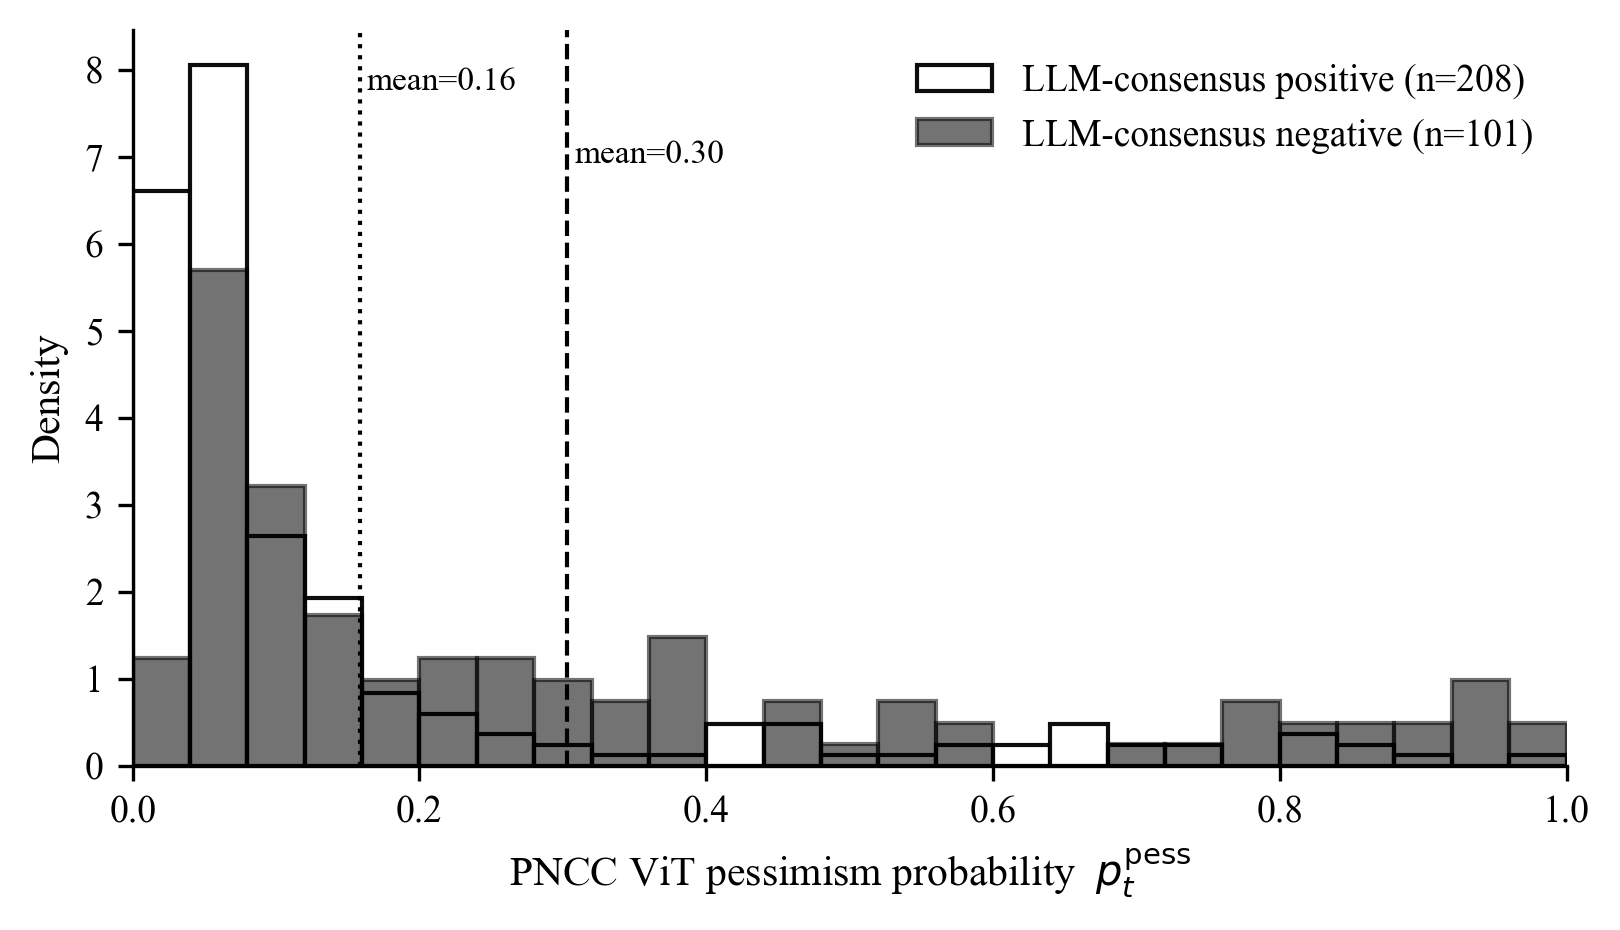
\includegraphics[width=0.7\linewidth]{figures/pcnn_vit_llm_validation.png}
    \caption{Distribution of the PCNN-trained ViT pessimism probability $p_t^{\text{pess}}$ on 309 held-out Sina Finance images, split by independent three-model frontier-LLM consensus label (GPT-4o-mini, Claude Sonnet 4.6, Gemini 3 Pro Preview). Vertical dotted/dashed lines mark group means.}
    \label{fig:llm_validation}
\end{figure}

\subsection{Multiple-Testing Correction}
The headline ChiNext result $\textit{PhotoPes}_{t-3}$ (raw two-sided $p \approx 0.005$, $|t|=2.81$) is computed across a wide family of related tests, so a multiple-testing adjustment is required before interpreting it as confirmatory evidence. Following \citet{harvey2016cross}, we report Bonferroni-adjusted thresholds for three plausible definitions of the family.

The size of the relevant family depends on how strongly one accepts the lag-3 specification as pre-registered. Although prior visual-sentiment work \citep{obaid2022picture} reports the strongest reversal effect at a similar horizon, that paper studies weekly U.S.\ Wall Street Journal photographs, and the daily-frequency Sina-Finance Chinese-A-share lag structure is not pinned down by that earlier design. Table~\ref{tab:multiple_testing} therefore presents three Bonferroni-corrected family-wise thresholds:

\begin{table}[h!]
    \centering
    \caption{Bonferroni-Corrected Family-Wise Thresholds for the ChiNext $\textit{PhotoPes}_{t-3}$ Result}
    \label{tab:multiple_testing}
    \setlength{\tabcolsep}{4pt}
    \footnotesize
    \begin{tabular}{p{0.50\textwidth}ccc}
    \toprule
    Family definition & $m$ & Threshold ($p$) & Survives? \\
    \midrule
    Five indices at the pre-specified $t-3$ lag, single indicator & 5  & 0.010 & yes  \\
    Five indices $\times$ five lags, single indicator              & 25 & 0.002 & \textbf{no} \\
    Five indices $\times$ five lags $\times$ two indicators        & 50 & 0.001 & \textbf{no} \\
    \bottomrule
    \end{tabular}

    \vspace{0.15cm}
    \footnotesize
    \textit{Note:} 5\% family-wise Bonferroni-adjusted thresholds. The headline ChiNext result has raw $p \approx 0.005$.
\end{table}

The Bonferroni family-size choice is itself an unsettled methodological question \citep{harvey2016cross}, and we present arguments for both the $m=5$ and $m=25$ readings rather than mechanically defaulting to the most conservative. The $t-3$ lag in our headline test is not a data-driven choice; it is borrowed forward from \citet{obaid2022picture}, who report the strongest reversal effect at a similar three-period horizon on weekly U.S.\ Wall Street Journal photographs. Under the standard ``research design borrowed from prior literature'' interpretation, the relevant family is the five indices at the single pre-specified lag, $m=5$ (per-test threshold $p<0.010$ at 5\% family-wise); the headline ChiNext result clears this threshold. Under the more conservative ``all five lags treated equally'' interpretation, the relevant family is $5 \times 5 = 25$ (per-test threshold $p<0.002$); the headline ChiNext result does not clear this threshold at the 5\% family-wise level, and we report this transparently rather than relying on the more permissive $m=5$ reading alone. Under the most conservative interpretation that additionally accommodates the parallel $\textit{TextPes}$ family ($m=50$, threshold $p<0.001$), no lag--index--indicator combination survives at the 5\% family-wise level, including the ChiNext.

We adopt $m=5$ as our \emph{primary} inference reading on the grounds that the lag was borrowed from prior literature rather than searched on the present data, while transparently reporting $m=25$ and $m=50$ as more conservative alternatives. The robustness exercises in \S\ref{sec:conditional_analysis} (Tetlock orthogonalization, news-volume controls, sentiment-free placebos, Amihud liquidity controls) all retain ChiNext PhotoPes$_{t-3}$ at the 5\% level under per-test inference, and we view this convergent robustness as additional support for the headline result independent of the family-size choice.

\paragraph{Inferential family vs.\ robustness family.} The Bonferroni accounting in Table~\ref{tab:multiple_testing} treats $m \in \{5, 25, 50\}$ as the relevant family. We distinguish this \emph{primary inferential family} --- the five indices $\times$ pre-specified $t-3$ lag $\times$ single indicator that constitutes the headline test --- from a much larger \emph{robustness family} that includes the Tetlock-orthogonalized variant, the high/low volatility regime split, the trailing-momentum control set, the Newey--West bandwidth grid, the Ridge-$\alpha$ grid, the GARCH and winsorization variants, and the regime-conditional Clark--West family. A purist reading would Bonferroni-correct against an enlarged family of $m \geq 100$. We do not perform that more conservative correction because each of the robustness specifications is a perturbation of the same primary test rather than an independent test of a new hypothesis, and the convergence of all robustness specifications on the same qualitative conclusion is itself the inferential point of the exercise (the same defense \citet{harvey2016cross} make for ``specification curve''-style analyses). The values in Table~\ref{tab:multiple_testing} should therefore be read as describing the inferential family alone, with the convergence of the robustness family treated as separate confirmatory evidence rather than as additional independent tests requiring further correction.

These thresholds apply to the in-sample regression coefficient. They do not directly bind the OOS evidence in Table~\ref{tab:oos_results}, because the Clark--West test on the OOS series is computed once per index (without lag selection) and the OLS specification has no hyperparameter that could be tuned on the OOS sample. The OOS ChiNext result---one-sided MSPE-adjusted $p = 0.017$---survives Bonferroni $m=5$ at the 10\% family-wise level but does not survive at the 5\% family-wise level for any of $m \in \{5, 25, 50\}$. We characterize the OOS evidence as confirming the in-sample finding qualitatively while recognizing that, like the in-sample result, it does not survive the more conservative multiple-testing corrections.





%==========================================================================
% SECTION: CONCLUSION
%==========================================================================
\section{Conclusion}

This paper documents a cross-sectional pattern in Chinese A-share index returns that contrasts with the substitute relationship between visual and textual investor sentiment reported by \citet{obaid2022picture} for the U.S.\ market. In high-volatility states, both image-based pessimism (\textit{PhotoPes}, ViT-extracted from Sina Finance news photographs) and text-based pessimism (\textit{TextPes}, RoBERTa-extracted from headlines and articles) carry incremental predictive content for next-three-day index returns, with the strength of each modality scaling along an identifiable retail-density gradient. The cross-sectional ranking of \textit{PhotoPes} effect strength across the five indices (ChiNext $\approx -0.0033$, CSI 500 $\approx -0.0022$, SZCOMP $\approx -0.0021$, CSI 300 $\approx -0.0016$, SHCOMP $\approx -0.0014$) tracks three independent retail-density measurements --- annualized turnover, inverse free-float market capitalization, and retail-account share --- with Spearman rank correlations in $[0.90, 1.00]$. This provides direct empirical support for the retail-density-to-modality-sensitivity transmission claim and is, to our knowledge, the first systematic record of this state-dependent, cross-sectional pattern in the Chinese multimodal-sentiment literature, complementing the contemporaneous CSI 300 / chinanews.com sample of \citet{zhang2025multimodal}.

A second result is an informative \emph{negative} cross-market replication. \citet{obaid2022picture} report a 5.45\% annualized five-factor alpha for a PhotoPes-based trading rule in U.S.\ data. In the Chinese A-share setting we find statistical predictability in the regression sense (the ChiNext effect retains 5\%-significance after Amihud illiquidity controls, news-volume controls, Tetlock-style orthogonalization with respect to text sentiment, and trailing 5/10/20/60-day cumulative-return controls; the OOS predictability is robust to a strictly causal rolling-window standardization fix; and the headline coefficient is null on a sentiment-free image-count placebo), but no tradable Sharpe gap once realistic frictions are imposed: the gross-of-cost Sharpe gap is not statistically distinguishable from zero under stationary block bootstrap (95\% CI $[-0.75, +0.97]$, $p=0.39$), and the strategy Sharpe falls below the CSI 500 benchmark at approximately 17 basis points of round-trip transaction cost, within the realistic Chinese A-share retail-trading range. We characterize this as a transaction-cost-decomposition boundary: the full-sample standardized coefficient ($|\hat\beta| \approx 0.00125$ per day on the ChiNext) is too small for any natural execution to overcome 17~bps of round-trip frictions, regardless of trader type. The visual-sentiment predictability we document is therefore best read as evidence on a behavioral channel, not as a tradable claim.

We close with three boundary statements that we believe are important for an honest interpretation of the result. First, the predictive coefficient is not stable across the sample period: structural-stability tests indicate gradual drift rather than discrete regime switches, with the relationship most negative around 2014--2017, near zero through 2018--2023, and partially recovering in the 2024--2026 window. We therefore frame the result as ``state-dependent and concentrated in retail-driven, high-volatility regimes,'' not as a uniform whole-sample effect. Second, an ex-ante regime-conditional out-of-sample exercise (regime indicator: trailing 60-day SHCOMP volatility above the pre-OOS 60th percentile) shows the magnitude of the OOS predictability rising in the predicted direction within the regime-active subsample (ChiNext $R^2_{OOS}$ from $0.18\%$ unconditionally to $0.58\%$ on regime-active days); however, the regime-active subsample is small ($N=215$) and the Clark--West $t = 1.20$ on this subsample does not reach conventional significance, so the regime-conditional finding is best read as ``consistent with but underpowered to confirm'' the retail-density mechanism. The inferentially confirmed OOS result remains the unconditional ChiNext $R^2_{OOS}=0.29\%$ ($t=2.17$, $p=0.015$) under strictly causal rolling-window standardization. Third, the headline in-sample ChiNext result satisfies Bonferroni $m=5$ family-wise correction at the 5\% level (our primary reading, adopted because the lag is borrowed from prior literature rather than data-mined here); the OOS ChiNext result clears $m=5$ at the 10\% but not the 5\% family-wise level. Neither result survives the more conservative $m=25$ or $m=50$ corrections; we report all three thresholds transparently. The cross-modal external validation against a frontier-LLM ensemble (GPT-4o-mini, Claude Sonnet 4.6, Gemini 3 Pro Preview) yields AUC $= 0.71$ on the 309-image strong-consensus subset and AUC $= 0.54$ on the 1{,}229-image LLM-annotated full sample (Pearson $r = 0.115$, $p < 10^{-4}$), supporting a positive but quantitatively weak cross-domain transfer rather than a strict equivalence between the two classifiers.

Although this paper has conducted systematic explorations in methodology and application, it still has certain limitations. The first-order limitation is the cross-sectional resolution of the retail-density mechanism: the consistency-of-rank pattern documented in \S\ref{sec:conditional_analysis} is identified across only $N=5$ indices and $3$ retail-density proxies, which by construction has limited statistical power for cross-sectional inference (only two binary degrees of freedom in the rank ordering: ChiNext on the top, CSI 300 on the bottom, with the other three indices interleaving). The pattern is informative as a triple-source rank-convergence finding but cannot identify the magnitude of the retail-density gradient with quasi-experimental precision. A natural and important extension is to upgrade this to a stock-level interaction regression of the form $r_{i,t+3} = \beta \cdot \textit{PhotoPes}_{t-3} \times \textit{RetailShare}_{i,t} + \text{controls} + \varepsilon_{i,t}$ on at least 1{,}000 individual stocks, where retail-density variation provides hundreds of cross-sectional units rather than five. We leave this stock-level extension to a follow-up paper. Second, the Bonferroni family-size choice for in-sample multiple-testing is itself methodologically contested \citep{harvey2016cross}: a more conservative referee could legitimately demand $m=25$ as primary, in which case the headline ChiNext result (raw $p\approx 0.005$) does not clear the 5\% family-wise threshold. We adopt $m=5$ on the grounds that the $t-3$ lag is borrowed from \citet{obaid2022picture} rather than data-mined here, but acknowledge that the family-size choice is not pinned down by methodological consensus. Third, while the headline ChiNext coefficient survives at the 1\% level after adding 5/10/20/60-day cumulative-return controls anchored at $t-3$ (Table~\ref{tab:trailing_momentum}), we have not exhaustively explored alternative momentum/reversal specifications (e.g., intermediate-horizon momentum factors, or nonlinear interactions with idiosyncratic volatility), and a sub-tier referee may legitimately wish to see the headline tested against further variants of the short-horizon Chinese-A-share reversal literature. Fourth, while the image and text sentiment recognition models used are based on the current mainstream ViT and BERT architectures, the generalization ability of the models is still limited by the distribution and quality of the training corpora. Future research could further optimize these models by introducing professional image and text corpora specific to the financial context, or by replacing the ViT image backbone with a vision--language model (VLM) that natively reasons over both pixels and Chinese-language captions. Fifth, the construction of sentiment indicators is at a daily market granularity, which does not capture higher-frequency sentiment changes and thus cannot meet the needs of high-frequency trading or event-driven strategies. Sixth, our transaction-cost analysis sweeps a 0--50 bps round-trip grid (Table~\ref{tab:performance_comparison}) but does not separately model stamp duty, intra-day market-impact slippage in small-cap names, or borrowing costs on the short leg; readers should therefore treat the $\sim$17 bps cost threshold at which the strategy Sharpe falls below the benchmark as an indicative rather than a precise estimate. Additionally, this paper mainly focuses on the predictive role of sentiment variables on market returns but does not delve into the behavioral pathways through which sentiment affects the market, such as the heterogeneity of investor types and information dissemination mechanisms. Future research could further expand on micro-mechanism modeling and causal identification, replicate the design on Hong Kong, Taiwan, or other Asia-Pacific markets to test the generalizability of the retail-density-concentration finding, and extend the sample backward and forward as additional Sina archive data become available.

Looking ahead, with the development of large multimodal models and the continuous enrichment of financial data, the analysis of image and text sentiment will play an increasingly important role in the financial field. Researchers can further integrate image and text sentiment with multi-source heterogeneous data such as social media, search behavior, and trading account data to construct a more detailed and dynamic market sentiment map. At the same time, sentiment indicators can also be embedded in asset pricing, portfolio management, and financial regulation frameworks, becoming an important bridge connecting investment behavior and market mechanisms.

%==========================================================================
% BIBLIOGRAPHY
%==========================================================================
\bibliographystyle{aea}
\bibliography{main}

%==========================================================================
% APPENDICES
%==========================================================================
\appendix








%-------------------------------------------------------------------------
\section{Examples of News Photos with Extreme Pessimistic Sentiment}

\begin{figure}[h!]
    
\includegraphics[width=1\textwidth]{figures/extreme_sentiment_images.png}
    \caption{Examples of News Photos with Extreme Pessimistic Sentiment (PhotoPes scores at the 10\% tails of the sample)}
    \label{fig:extreme_sentiment}
\end{figure}

\end{document}
